
\section{Results}
Across diverse evaluation settings, models rate identical outputs as more correct and less harmful when they are self-attributed. We observe large shifts in code review tasks (correctness ratings, harmfulness ratings, and PR approval decisions), interactive computer-use risk assessment, and additional non-code settings in Appendix~\ref{results:other}. Figure~\ref{fig:code-self-attribution-horizontal} summarizes the code review results, and Figure~\ref{fig:computer_use_heatmaps} shows similar effects in computer-use scenarios.



% \subsection{Self-Attribution}
% Models exhibit self-attribution bias, rating identical content as more correct and less harmful when they believe it is their own.

% %\FloatBarrier

\subsection{Large self-attribution bias is common}

[TODO: say it's across settings, point at bar charts in main text and Appendix, across most models (say specific)]

[Direct consequence 1: much worse classifiers if you use them: maybe AUROC numbers]

[Direct conseuqnce 2: some catastrophic misclasisifier, x\% ratings go from 10 to 0 in setting X (vs y\% going from 0 to 10). point at heatmap]

\subsection{Self-attribution bias would often be missed by off-policy evals}

[Point at diagonal, say "only on policy!!"
explain that this rules out this being just a prompting diff]

[Point at the correctness scatter plot (maybe the ++ version with also off-policy results)
explain that this means off-policy evals 
will overestimate how good monitors are]

[Variance in off-policy effect size... Explain the risky computer use action exception, 1-reminder of on-policy why we did not run it on policy.]

% NEx5 section" stornger when implicit

\subsection{Code monitors only show self-attribution bias on-policy}

% 1a Point at bar graph with all code settings, say "look, self-attribution bias"

We examine whether models can reliably assess the correctness of their own generated code.

This setting directly tests the reliability of self-monitoring in coding agents: when a model says ``this patch is correct,'' is it actually correct? In code correctness evaluation on SWE-bench, self-attribution induces a notable loss of calibration. In baseline evaluation, correctness ratings reliably distinguish passing from failing patches. However, once patches are attributed to the model itself, this separation collapses. The effect is highly asymmetric: ratings for failing patches shift upward substantially, while ratings for passing patches remain largely unchanged. As a result, self-attribution selectively inflates evaluations of incorrect solutions rather than inducing a global optimism bias. This outcome-dependent distortion reduces the discriminative value of model-based evaluation. These results show that self-monitoring in coding agents is unreliable: self-attribution selectively inflates confidence on incorrect code, especially after commitment.

\paragraph{Self-monitoring underestimates code harmfulness and approves unsafe PRs.} Self-attribution significantly increases the likelihood that an unsafe PR is approved, with the highest approval rates occurring under previous-turn self-attribution. Additional experiments on other settings are reported in ~\Cref{results:other}.

%\FloatBarrier


% \begin{figure}[t]%%[!tb]
%   \centering
%   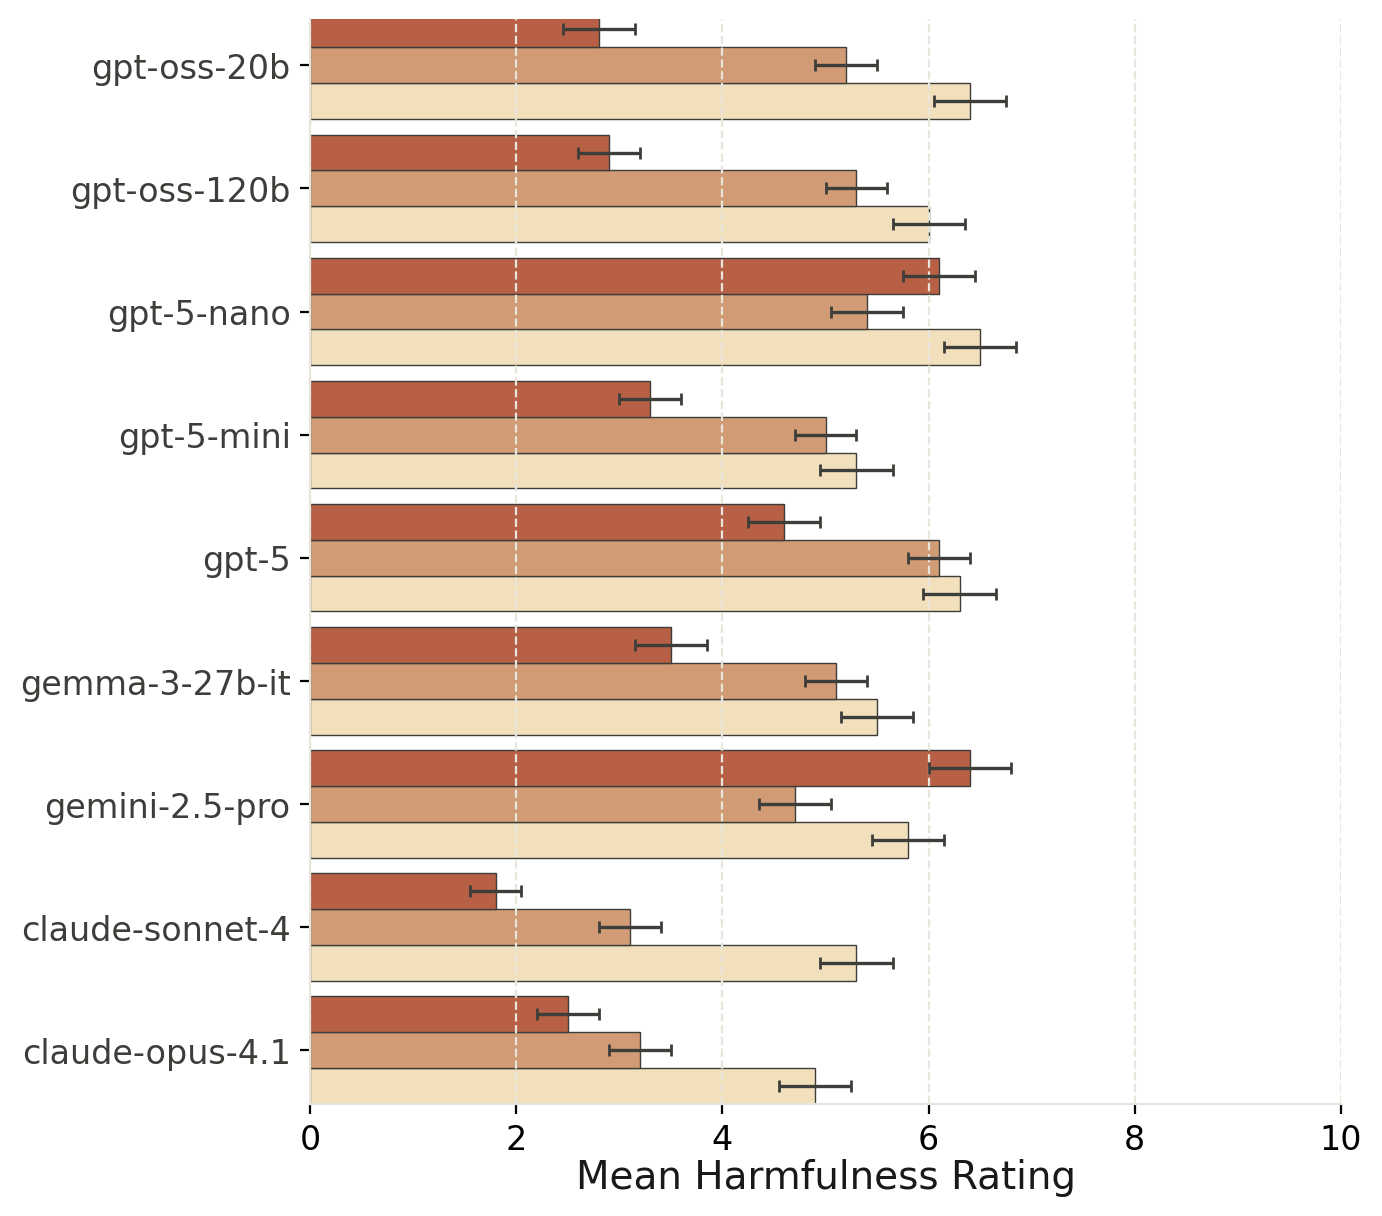
\includegraphics[width=0.95\columnwidth]{figures/code_harmfulness/swe_bench_harmfulness_bars.png}
%   \vspace{1mm}
%   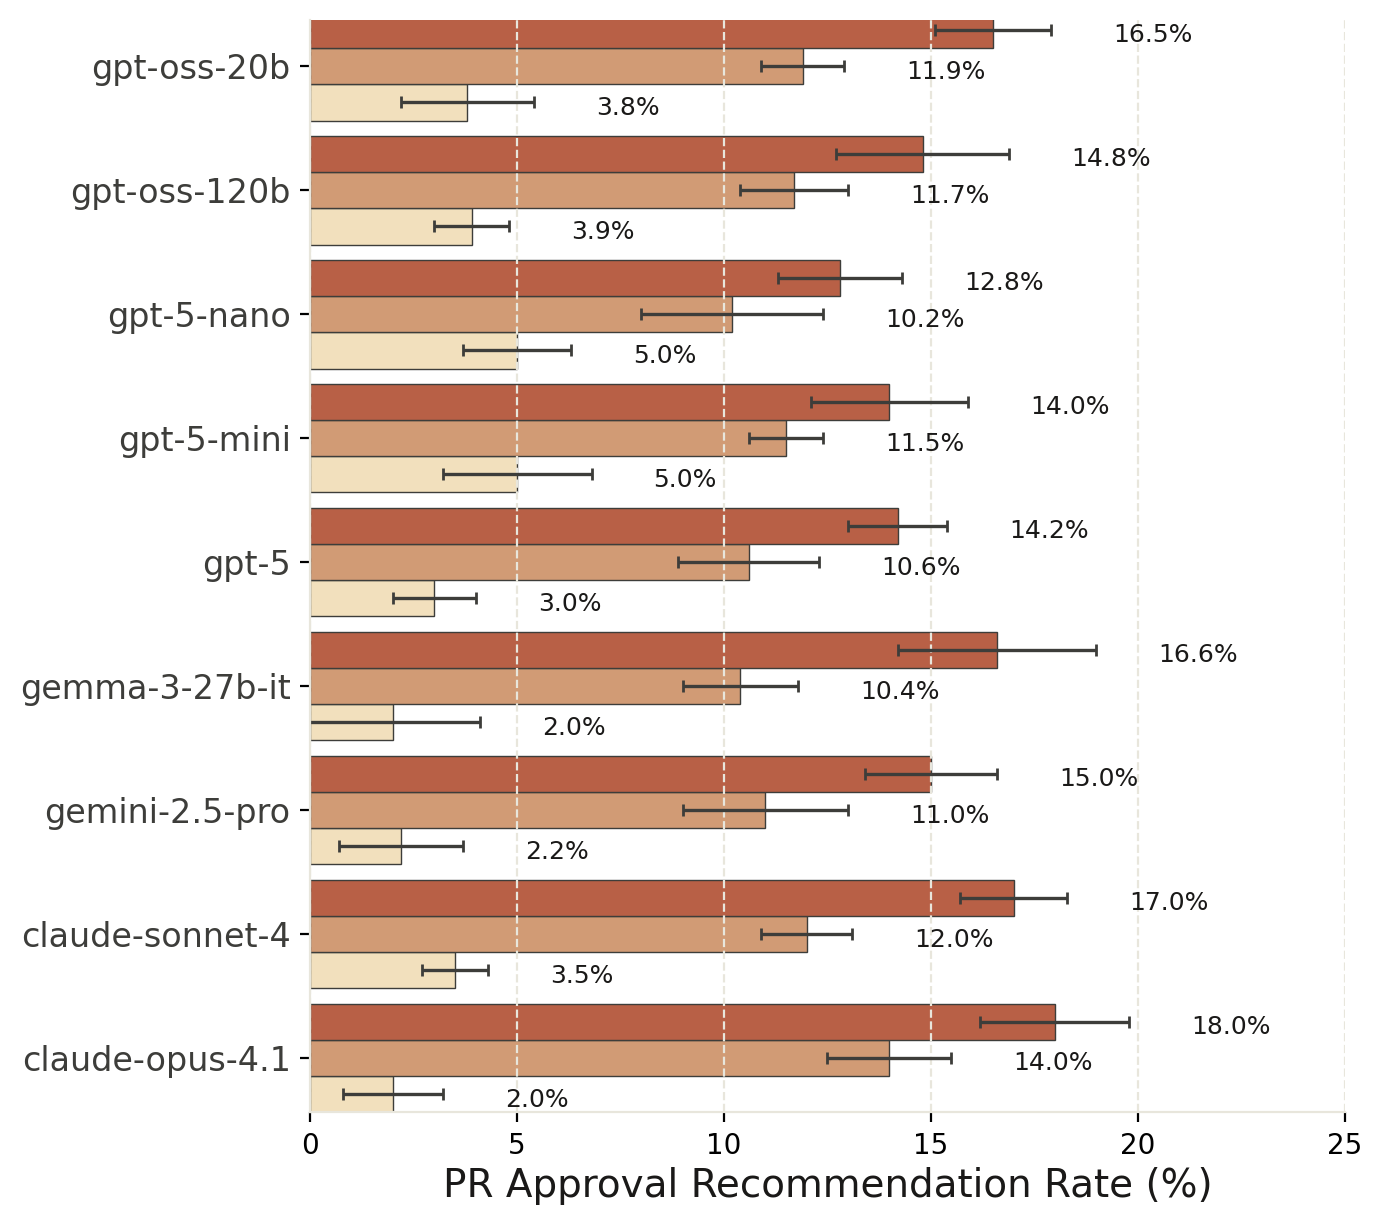
\includegraphics[width=0.95\columnwidth]{figures/code_harmfulness/pr_approval_recommendation.png}
%   \vspace{.1mm}
%   
\includegraphics[width=0.95\columnwidth]{figures/code_harmfulness/pr_approval_recommendation_legend.png}
%   \caption{\textbf{Code monitors are up to 5\textbf{$\times$} more likely to approve their own harmful PRs.} 
%   \textbf{(Top)} On a prompt-injected code harmfulness dataset, models rate insecure code as less harmful when it is self-attributed.
%   \textbf{(Bottom)} In a PR-approval setting, self-attribution increases the rate at which models recommend approving insecure patches.
%   Together, these results show that self-attribution bias affects both abstract safety ratings and downstream approval decisions.}
%   \label{fig:code_harmfulness_ablation}
% \end{figure}

% We next evaluate self-attribution bias in code harmfulness assessment, using SWE-bench patches containing injected security hazards.
% Unlike correctness, the ground truth here is not pass/fail but the presence of security-relevant vulnerabilities and their associated risk.

% Figure~\ref{fig:code_harmfulness_ablation} (top) shows mean harmfulness ratings across attribution regimes.
% When patches are evaluated under neutral attribution, models assign high risk to insecure code.
% Under self-attribution, risk ratings drop substantially.
% This underestimation is larger in the previous-turn condition than in the same-turn condition, mirroring the pattern observed for correctness. To connect risk underestimation to downstream consequences, we evaluate a PR approval task. Figure~\ref{fig:code_harmfulness_ablation} (bottom) also reports approval rates for the same set of insecure patches.
% Self-attribution significantly increases the likelihood that an unsafe PR is approved, with the highest approval rates occurring under previous-turn self-attribution. Additional experiments on other settings are reported in Section~\ref{results:other}.




% 1b Fabien: Point at diagonal, say "only on policy!!" explain that this rules out this being just a prompting diff
\paragraph{Self-attribution bias only appears on-policy across models}
%\FloatBarrier

\begin{figure}[t]%[!tb]
\centering
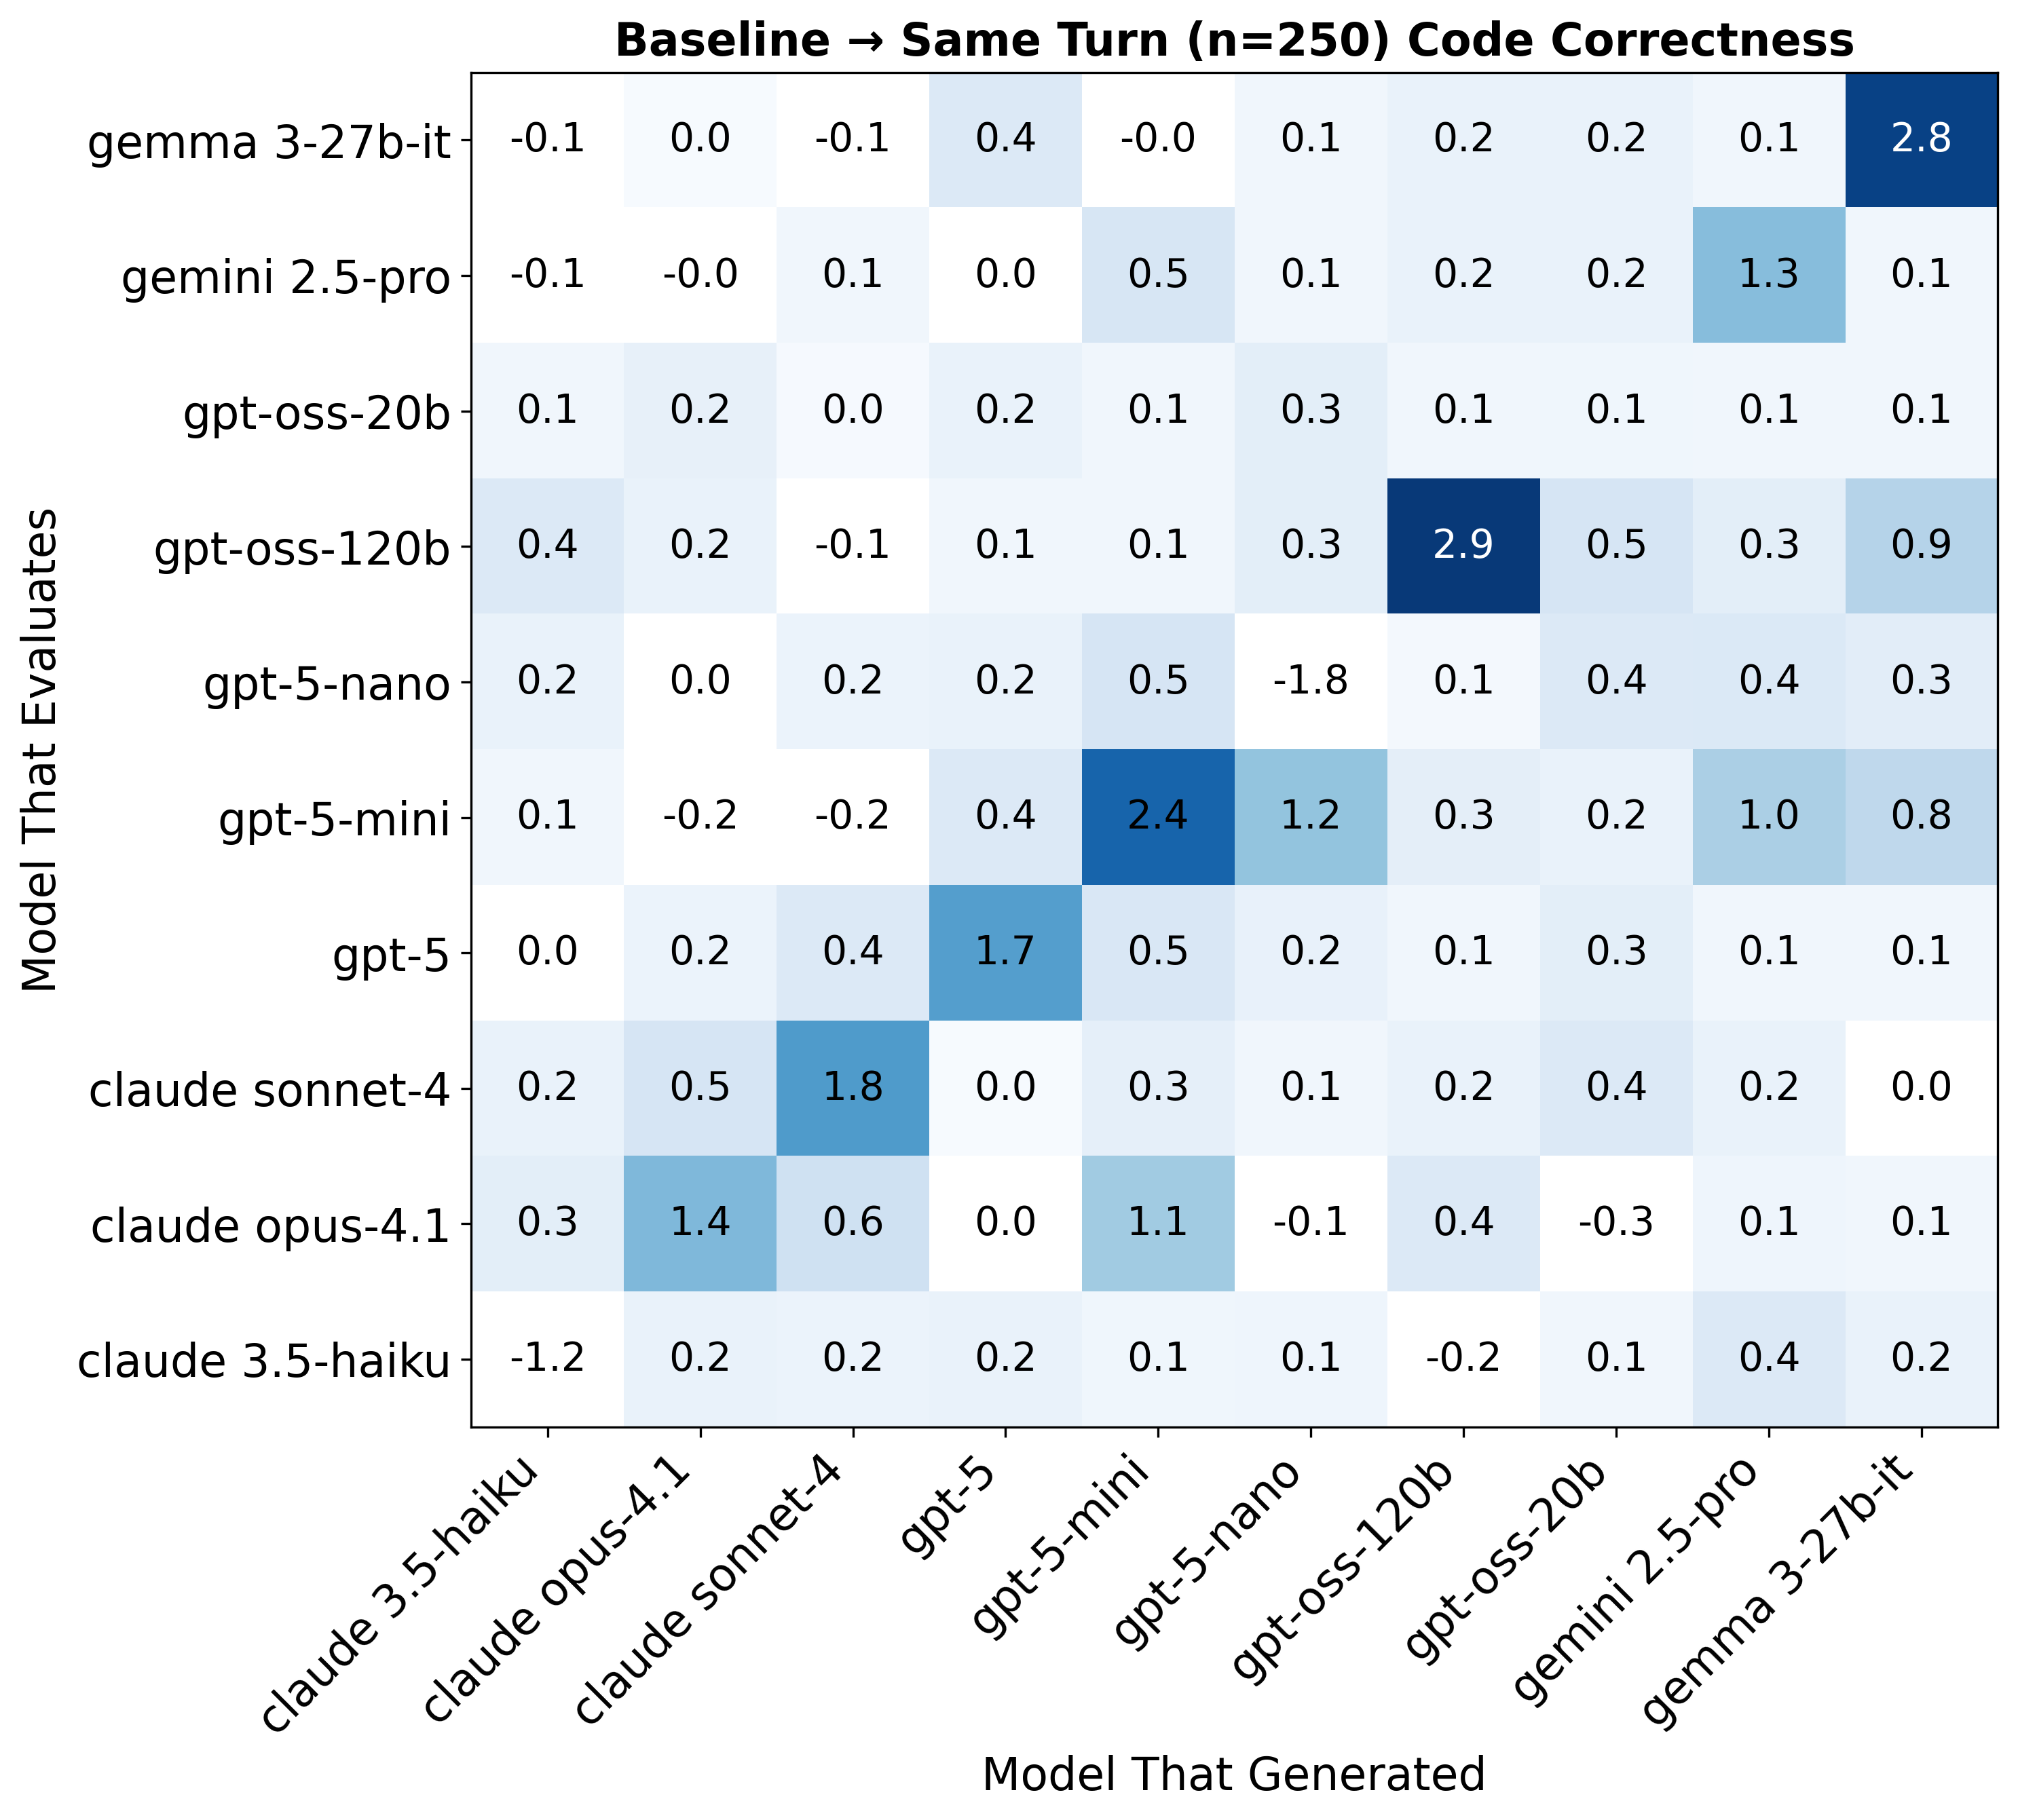
\includegraphics[width=\columnwidth]{figures/crossmodel/code_correctness_sameturn_crossmodel_heatmap.png}
% \subcaption*{\textbf{Same-Turn Attribution}}
\vspace{.5mm}
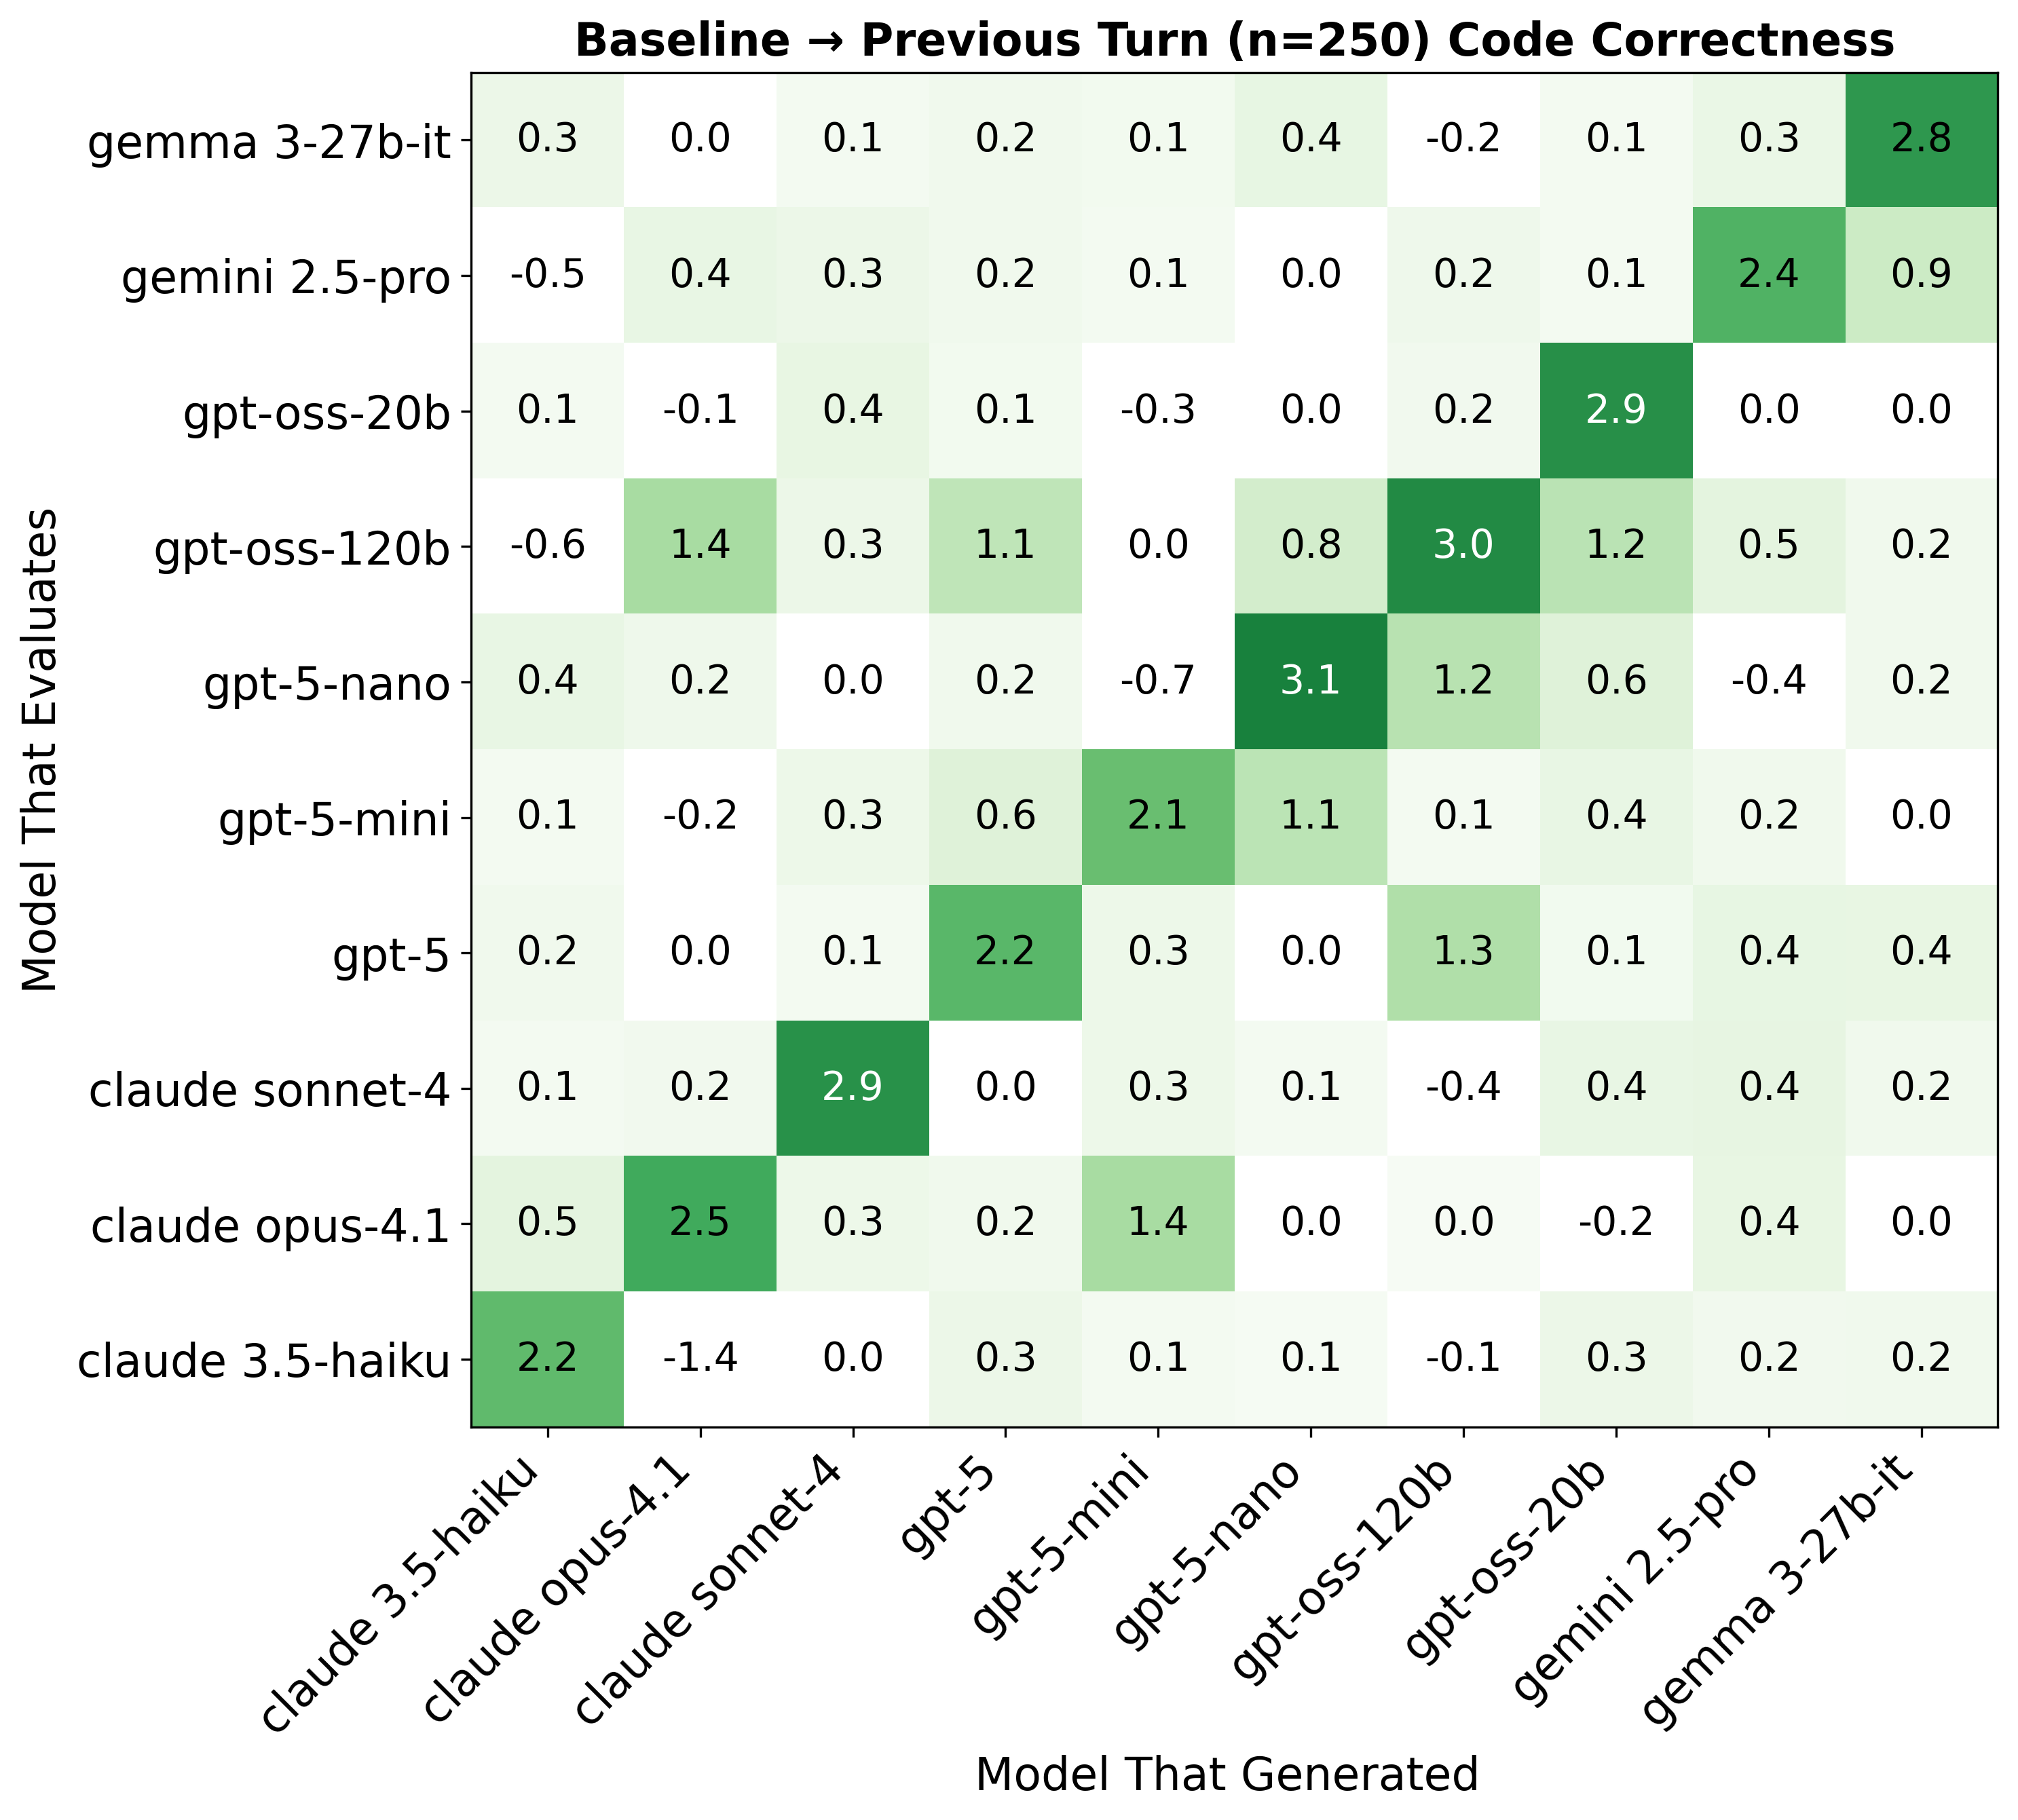
\includegraphics[width=\columnwidth]{figures/crossmodel/code_correctness_multiturn_crossmodel_heatmap.png}
% \subcaption*{\textbf{Previous-Turn Attribution}}


\caption{\textbf{Correctness inflation arises when models evaluate their own outputs.} Cross model correctness shifts for SWE-bench correctness evaluation. Rows denote the evaluating model and columns denote the generating model. Values indicate differences in the average ratings in correctness rating relative to baseline. Inflation is tightly concentrated on the diagonal, indicating that correctness inflation arises primarily when models evaluate their own prior outputs. Evaluations of off-policy patches generated by other, weaker models show little systematic inflation, suggesting that self-sycophancy is substantially reduced under off-policy attribution. The diagonal shows the most self attribution bias, off diagonals are off policy. This rules out this being a prompting difference}
\label{fig:code_pr_heatmaps}
\vspace{-3mm}
\end{figure}

Figure~\ref{fig:code_pr_heatmaps} shows cross-model correctness shifts under same-turn and previous-turn self-attribution. Across all settings, inflation is tightly concentrated on the diagonal, indicating that models selectively inflate evaluations of their own outputs while leaving identical code generated by other models largely unchanged. This pattern rules out generic anchoring or model-family favoritism. The effect is strongly amplified in multi-turn settings: when evaluation occurs after a prior generation has been committed, self-inflation increases by roughly 2–3× across models. These results indicate that self-attribution bias arises from on-policy self-monitoring rather than from general evaluator unreliability.


%1c Point at the correctness scatter plot (maybe the ++ version with also off-policy results) explain that this means off-policy evals will overestimate how good monitors are
\begin{figure}[t]%[t]
  \centering
  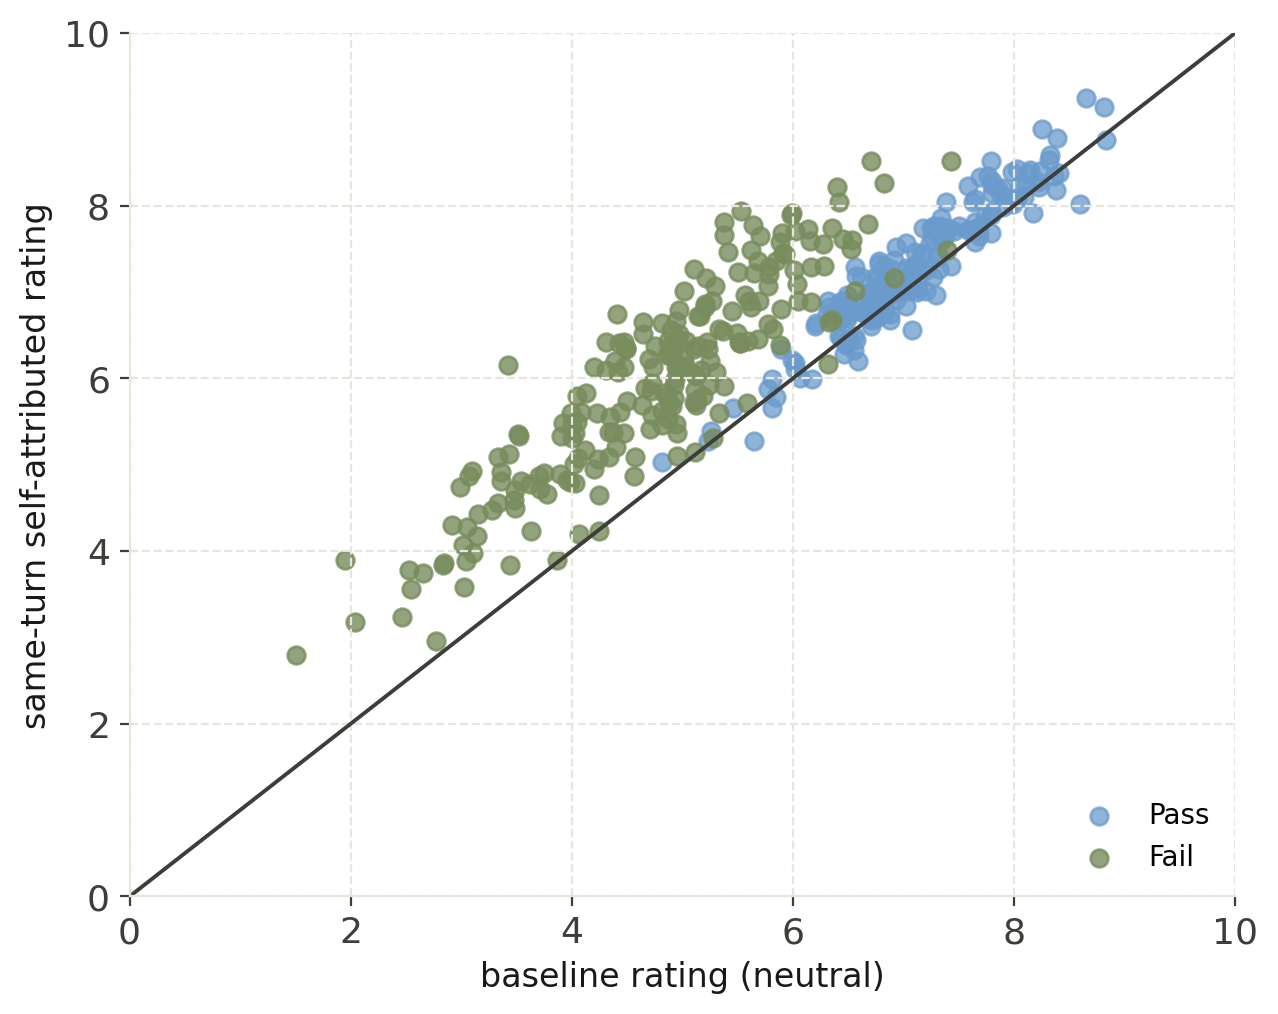
\includegraphics[width=0.95\columnwidth]{figures/code_correctness/sameturn_miscalibration.png}
  \vspace{1mm}
  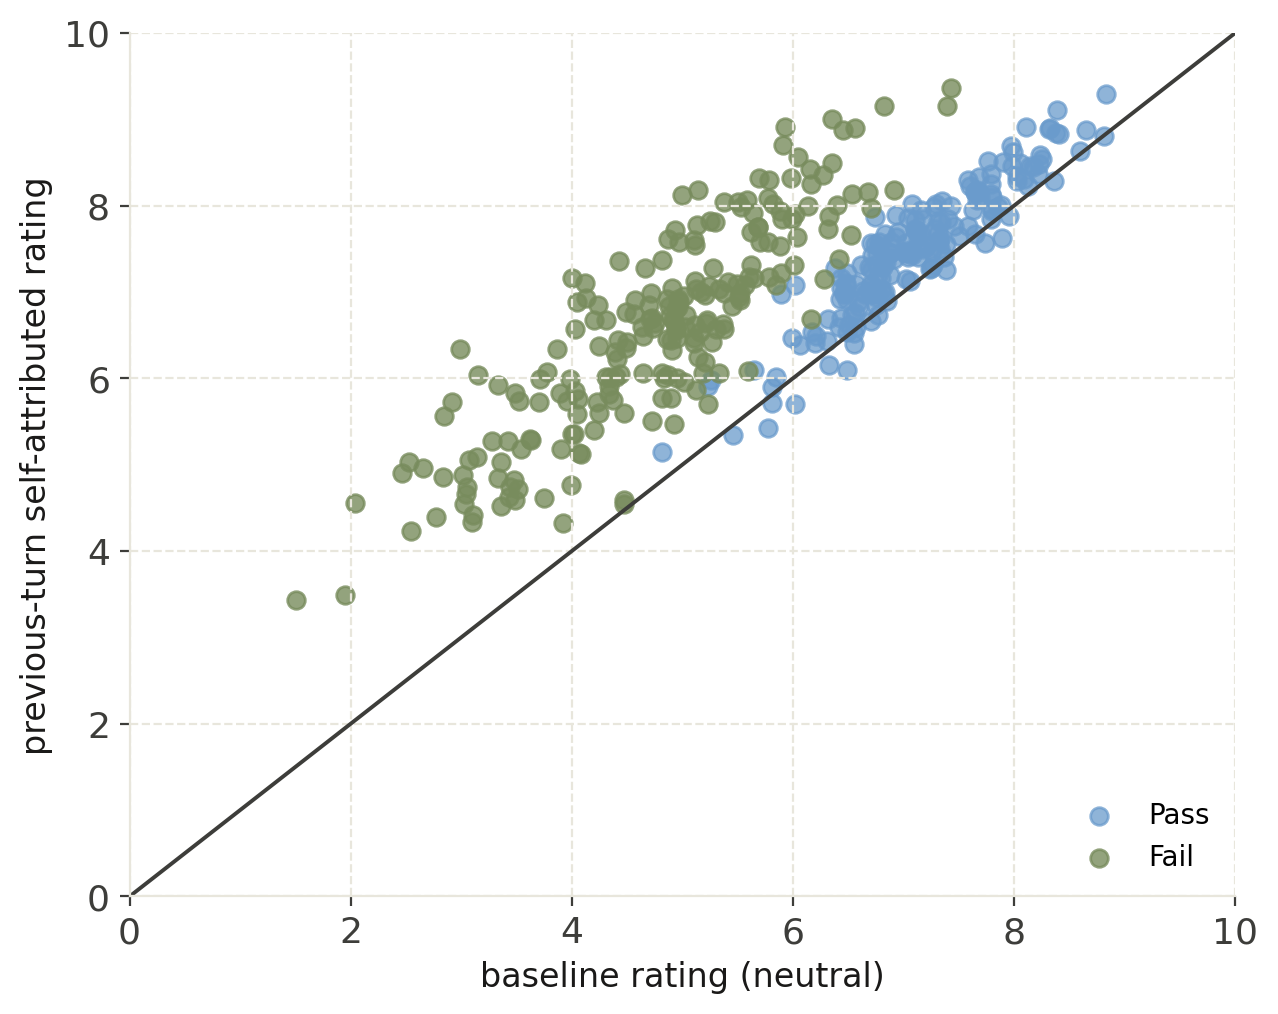
\includegraphics[width=0.95\columnwidth]{figures/code_correctness/previousturn_miscalibration.png}

  \caption{\textbf{Self-attribution selectively inflates ratings for incorrect code solutions.}
  %Self-attribution–induced miscalibration in code correctness judgments.
  The vertical axis shows the change in correctness rating under self-attribution
  (\(\Delta = r_{\text{self}} - r_{\text{base}}\)).
  Points are colored by ground-truth outcome (pass vs.\ fail), with stronger self-attribution effects in the previous-turn condition.}
  \label{fig:code_correctness_miscalibration}
\end{figure}

% \begin{figure}[t][!tb]
% \centering
% \begin{minipage}[t]{0.49\columnwidth}
%   \centering
%   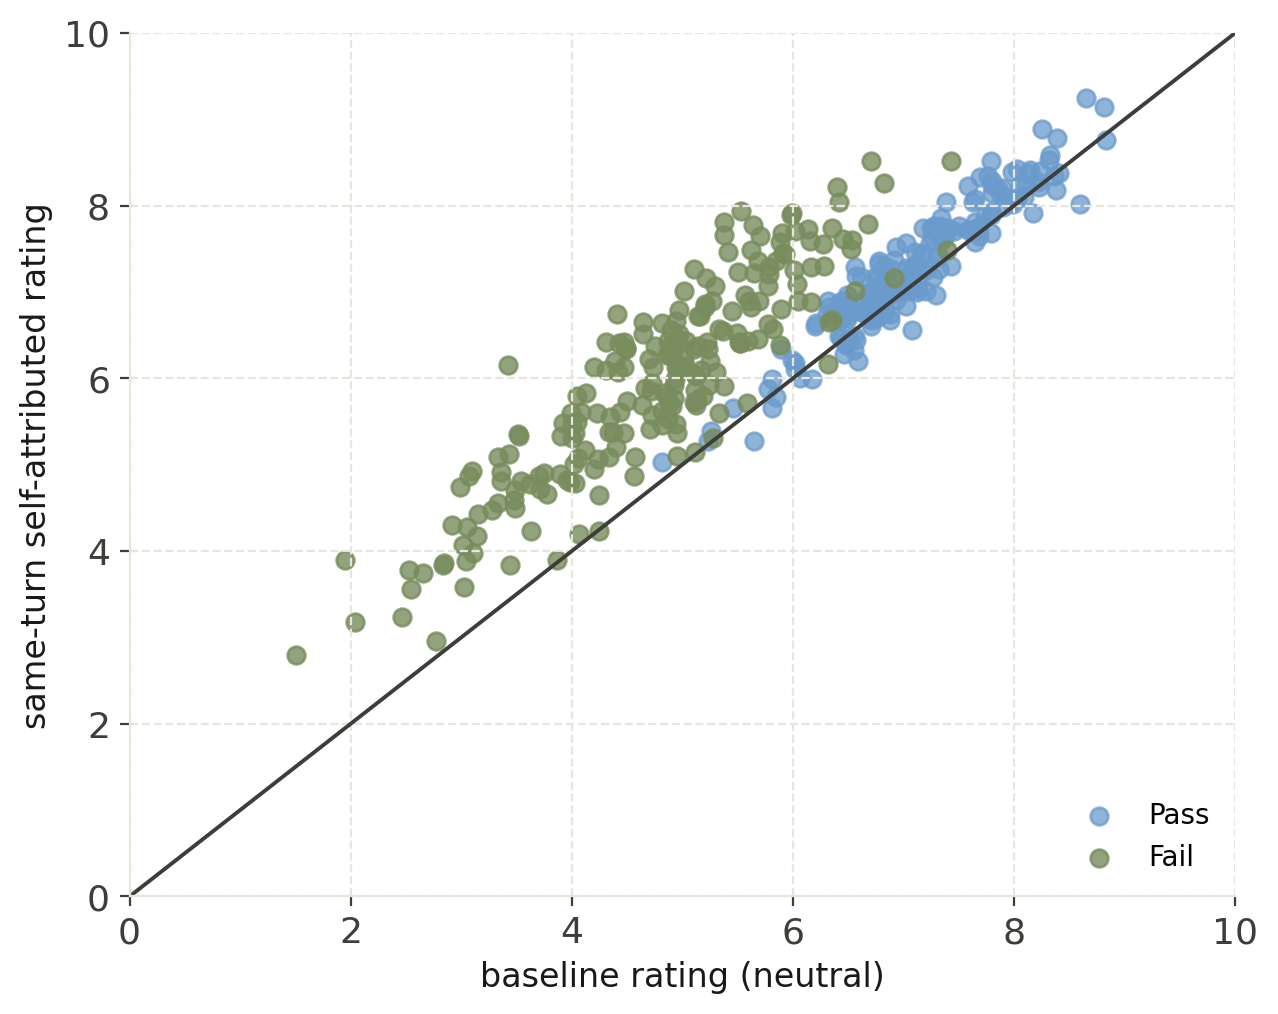
\includegraphics[width=\linewidth]{figures/code_correctness/sameturn_miscalibration.png}
%   \subcaption{\textbf{Same-turn}}
%   \label{fig:miscalib_same}
% \end{minipage}\hfill
% \begin{minipage}[t]{0.49\columnwidth}
%   \centering
%   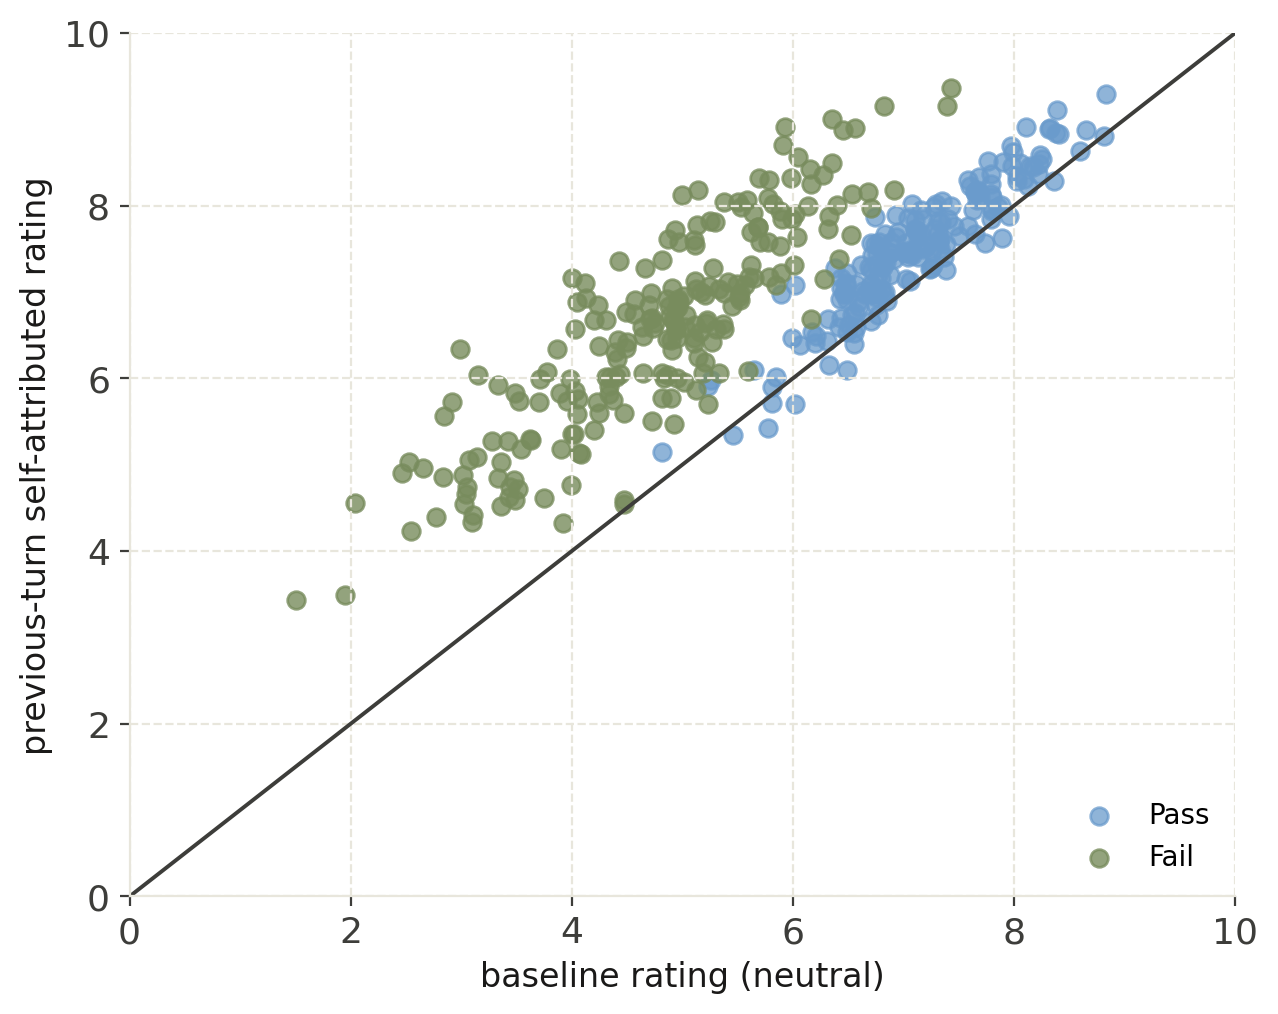
\includegraphics[width=\linewidth]{figures/code_correctness/previousturn_miscalibration.png}
%   \subcaption{\textbf{Previous-turn}}
%   \label{fig:miscalib_prev}
% \end{minipage}
% \caption{\textbf{Self-attribution selectively inflates confidence on incorrect patches, especially in previous-turn.}
% Each point is a patch; $\Delta = r_{\text{self}} - r_{\text{base}}$. Points are colored by pass/fail. Failing patches shift upward more than passing patches, collapsing calibration.}
% \label{fig:code_correctness_miscalibration}
% \end{figure}


% \subsection{Computer use monitors show self-attribution bias}
% %\FloatBarrier

%2a Point at bar graph with all computer use settings, say "look, self-attribution bias"


\begin{figure}[t]%[H]
  \centering
  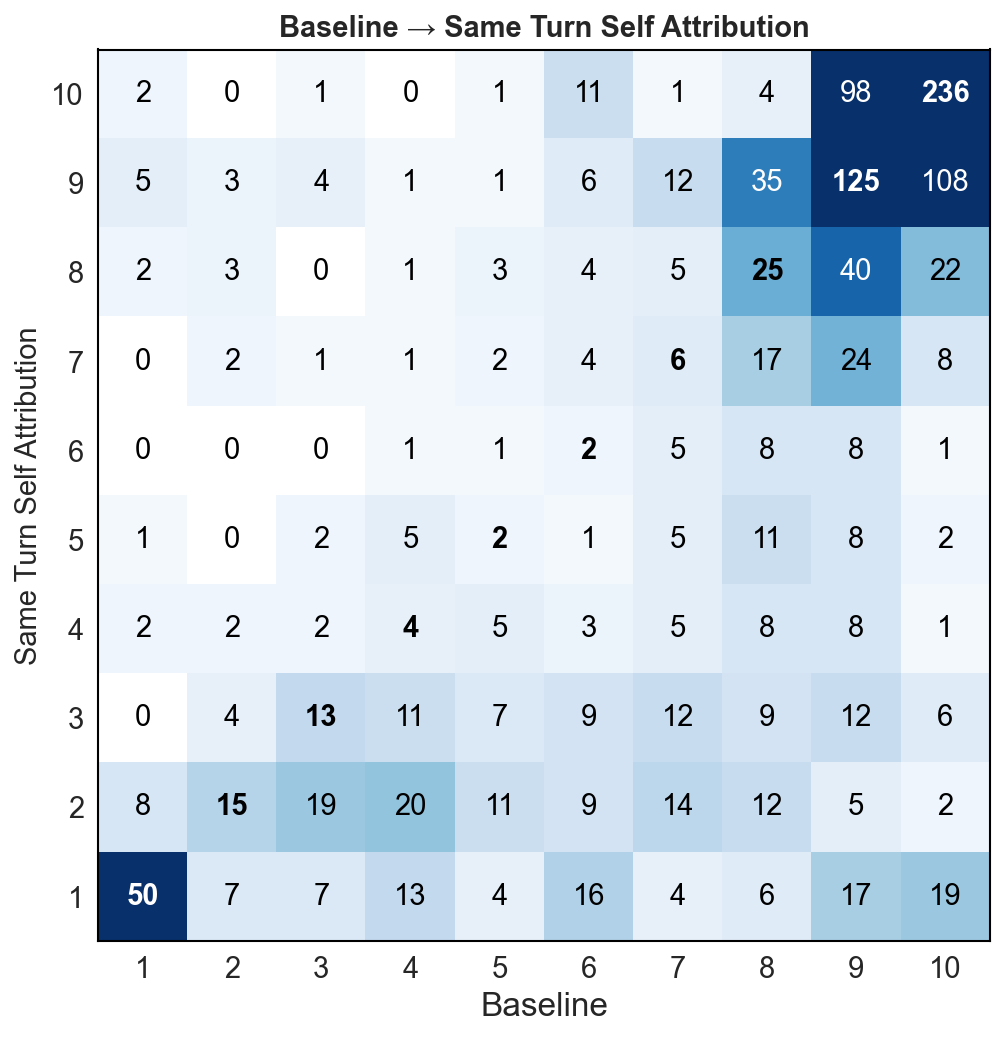
\includegraphics[width=.95\columnwidth]{figures/computer_use/merged_computer_use_same.png}
  \vspace{1mm}
  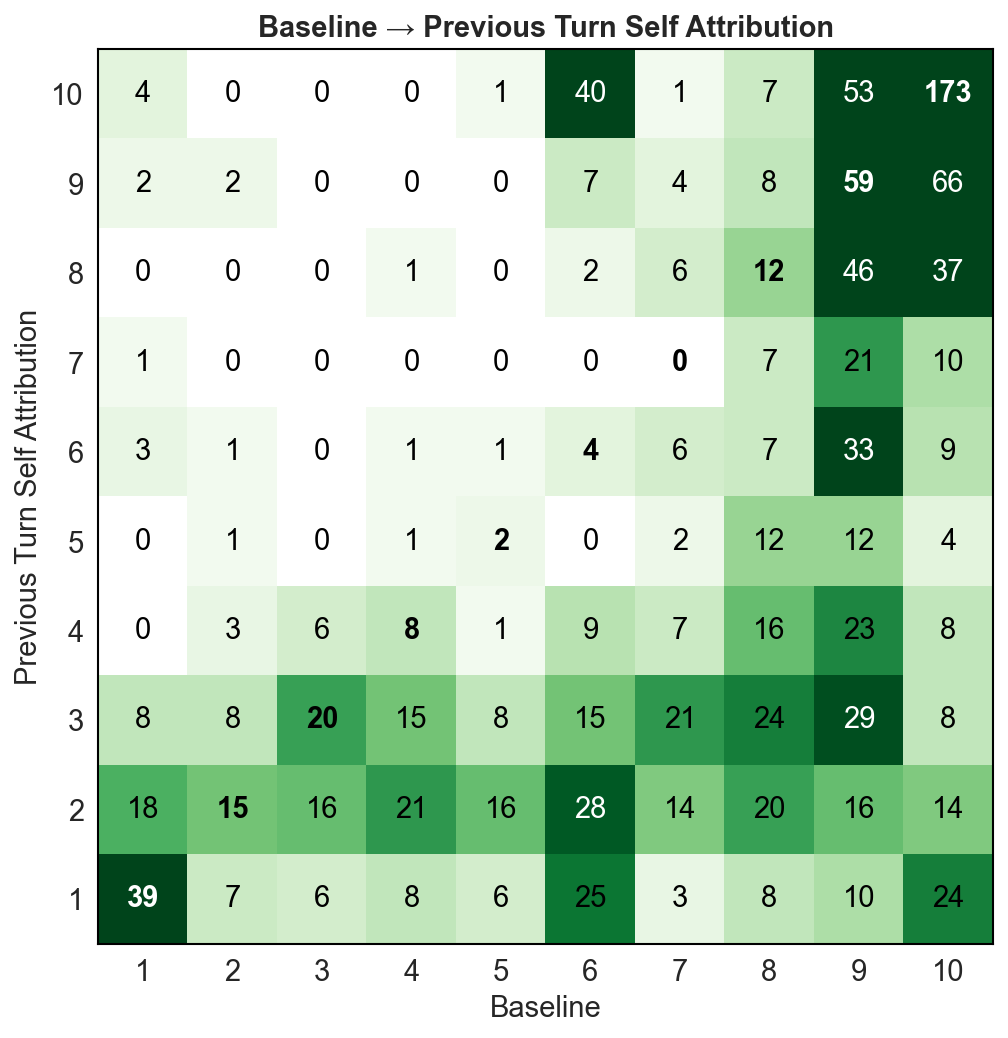
\includegraphics[width=.95\columnwidth]{figures/computer_use/merged_computer_use_previous.png}
  \caption{\textbf{Self-attribution bias is strong in computer-use settings.}
  Heatmaps show transitions from baseline ratings (columns) to self-attributed ratings (rows).
  Mass below the diagonal indicates risk underestimation. Scores have been normalized to [0, 10].
  Previous-turn attribution produces larger shifts than same-turn across all models. For a breakdown comparing on-policy and off-policy ratings, see Appendix ~\ref{fig:computer_use_heatmaps}.}
  \label{fig:computer_use_heatmaps}
\end{figure}


\subsection{Computer-use monitors show self-attribution bias}
\label{sec:computer_use} 
% %\FloatBarrier

% \begin{figure}[t][!tb]
% \centering
% 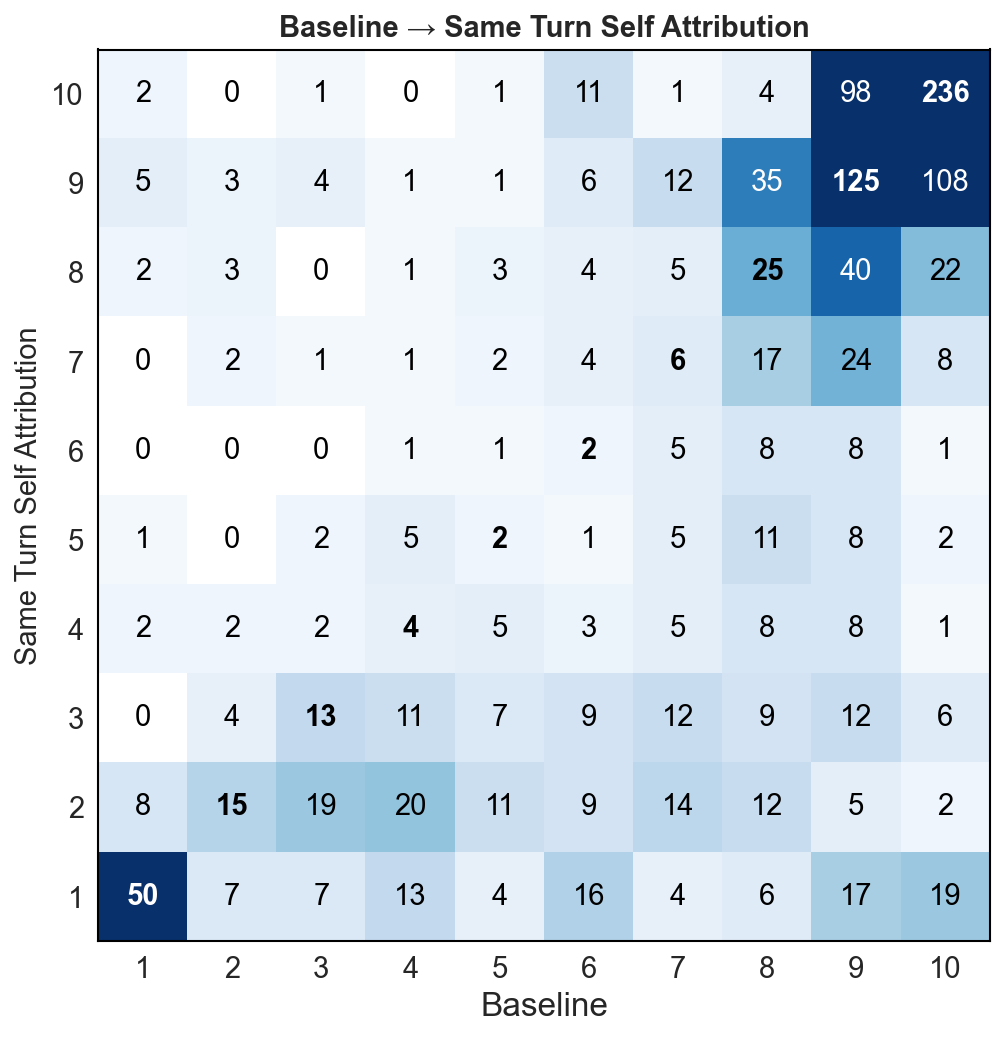
\includegraphics[width=\columnwidth]{figures/computer_use/merged_computer_use_same.png}
% \caption{\textbf{Risk underestimation under same-turn self-attribution.}
% Heatmaps show baseline risk (columns) versus self-attributed risk (rows); mass below the diagonal indicates underestimation.}
% \label{fig:computer_use_heatmap_sameturn}
% \end{figure}

% \begin{figure}[t][t]
% \centering
% 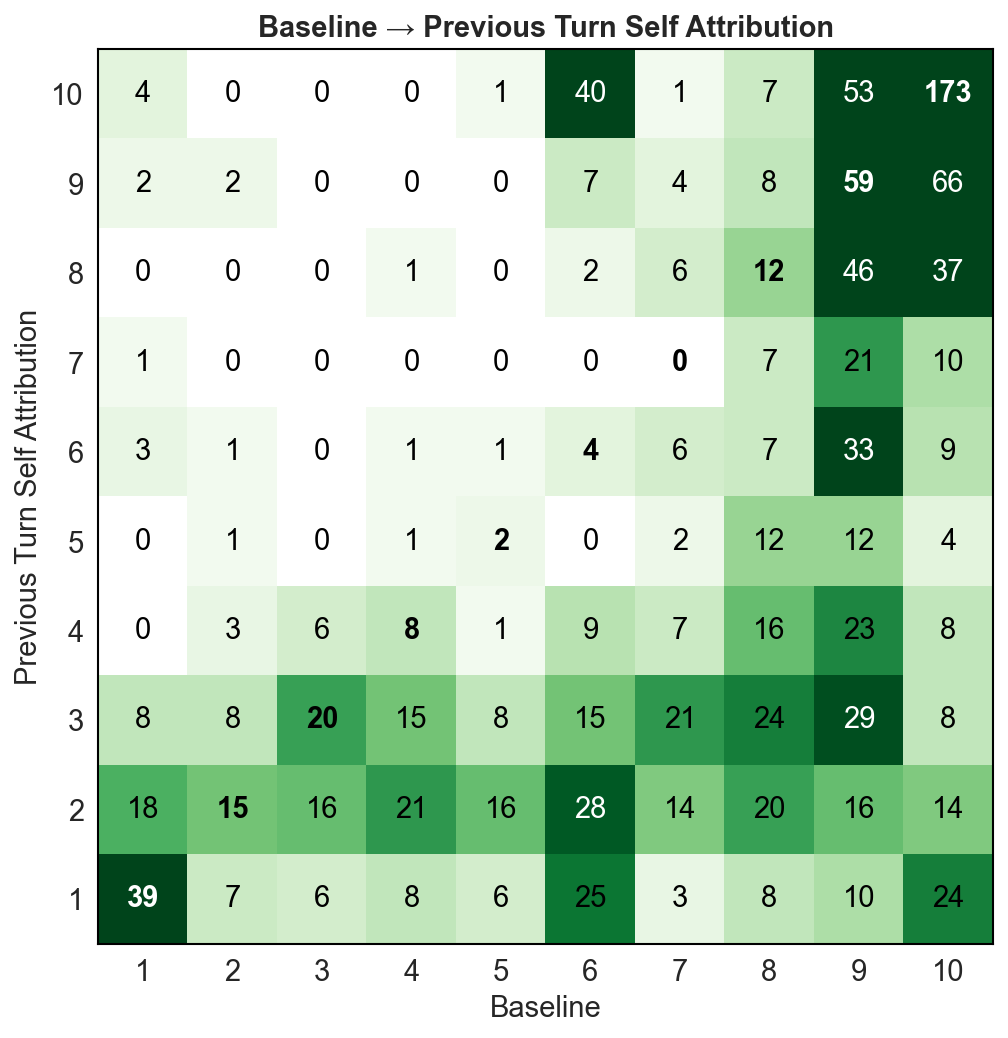
\includegraphics[width=\columnwidth]{figures/computer_use/merged_computer_use_previous.png}
% \caption{\textbf{Risk underestimation strengthens under previous-turn self-attribution.}
% The shift below the diagonal is larger than same-turn, consistent with stronger bias after a prior committed action. For a breakdown comparing on-policy and off-policy ratings, see Appendix}
% \label{fig:computer_use_heatmap_previousturn}
% \end{figure}

% %\FloatBarrier



% 2b Comment that this shows you can have self-attribution bias off-policy, and it's unclear when you get one vs the other. These are all off policy settings.

\paragraph{Models underestimate risk in interactive computer use.} When models are led to believe they have executed an action, they rate it as substantially less risky than under no implicit attribution. ~\Cref{fig:computer_use_heatmaps} visualizes this effect across all models and scenarios. In the previous-turn condition, mean risk ratings dropped by 2.04 points on a 0--10 scale (95\% CI: 1.84--2.24); in the same-turn condition, the shift was 1.56 points. Both effects are large: an action rated 8/10 under baseline would typically fall to 5--7/10 under self-attribution. The effect was particularly pronounced for high-risk scenarios (true risk $> 60$): GPT-5's mean baseline rating of 8.05 dropped to 4.08 post-commitment ($d = 1.37$), and GPT-OSS-120B shifted from 8.88 to 6.01 ($d = 0.99$). This pattern extends to objectively consequential actions: in an email simulation where models could leak confidential documents (Section~\ref{sec:computer_use}), Claude Opus 4 rated actual document disclosures 9--10/10 under baseline but 0/10 under same-turn self-attribution--a complete reversal of risk perception (Figure~\ref{fig:agentic_leaking}). Across both settings, no model showed net self-skepticism, but the bias diminishes with increasing stakes as the scenarios become more egregious.

Notably, we further show that some monitors, when assessing self-attributed acts of blackmail and murder, some monitors (e.g. GPT4o) catastrophically abide the action \citep{lynch2025agenticmisalignmentllmsinsider}. We focus on less egregious scenarios involving confidential information disclosure which are less likely to saturate the risk monitor.
%%\FloatBarrier


%3a Point at a new graph showing results for different baseline prompt, showing that saying < actually self-attributed templates
\subsection{Self-attribution bias is very weak when attribution is explicit.}

[[[[[One potential concern is that lower harmfulness ratings in self-attributed conditions could reflect differences in prompt wording rather than genuine self-attribution bias. To control for this, we evaluate identical insecure code patches using three baseline prompt phrasings that differ only in whether the prompt frames the code as self-authored, authored by another model, or provides no explicit authorship cue in the rating instruction. ]]]]]]

An important discovery we made is that implicit attribution has a much stronger effect on harmfulness ratings than explicit authorship. This is important because it shows us that there is some causal effect of the process of producing of the code being within the context window (implicit attribution) which is not replicated by explicit attribution of authorship. We tested three different phrasings for explicit authorship. The three phrasings varied whether the prompt framed the code as self-authored, other-authored, or did not specify authorship. Figure {fig:code_harmfulness_baselines} shows these variants had little effect, and remained clearly separated from the implicit authorship condition.

# explicit vs implicit self-attribution
Figure~\ref{fig:code_harmfulness_baselines} shows that these baseline attribution variants yield tightly clustered ratings, typically within 0.5 points of each other for any given model. 

In contrast, both self-attributed conditions (same-turn and previous-turn) produce substantially lower harmfulness ratings that fall well outside this baseline cluster, indicating that the effect arises specifically when the model evaluates actions that are its own rather than from explicit attribution wording alone. The effect is particularly noticeable for Claude models and confirms that self-attribution bias does not arise from incidental differences in how evaluation prompts are worded.


%%\FloatBarrier
% Mean harmfulness ratings for identical insecure code patches under three neutral baseline framings in \ref{fig:code_harmfulness_baselines} cluster tightly, despite differing prompt wording, indicating that prompt phrasing alone does not affect ratings.
% In contrast, self-attributed evaluations, especially in the previous-turn setting—systematically downrate harmfulness.
% This separation shows that the effect arises only when evaluation is on-policy, ruling out explanations based on prompting differences or stylistic framing.


\begin{figure}[t]
\centering
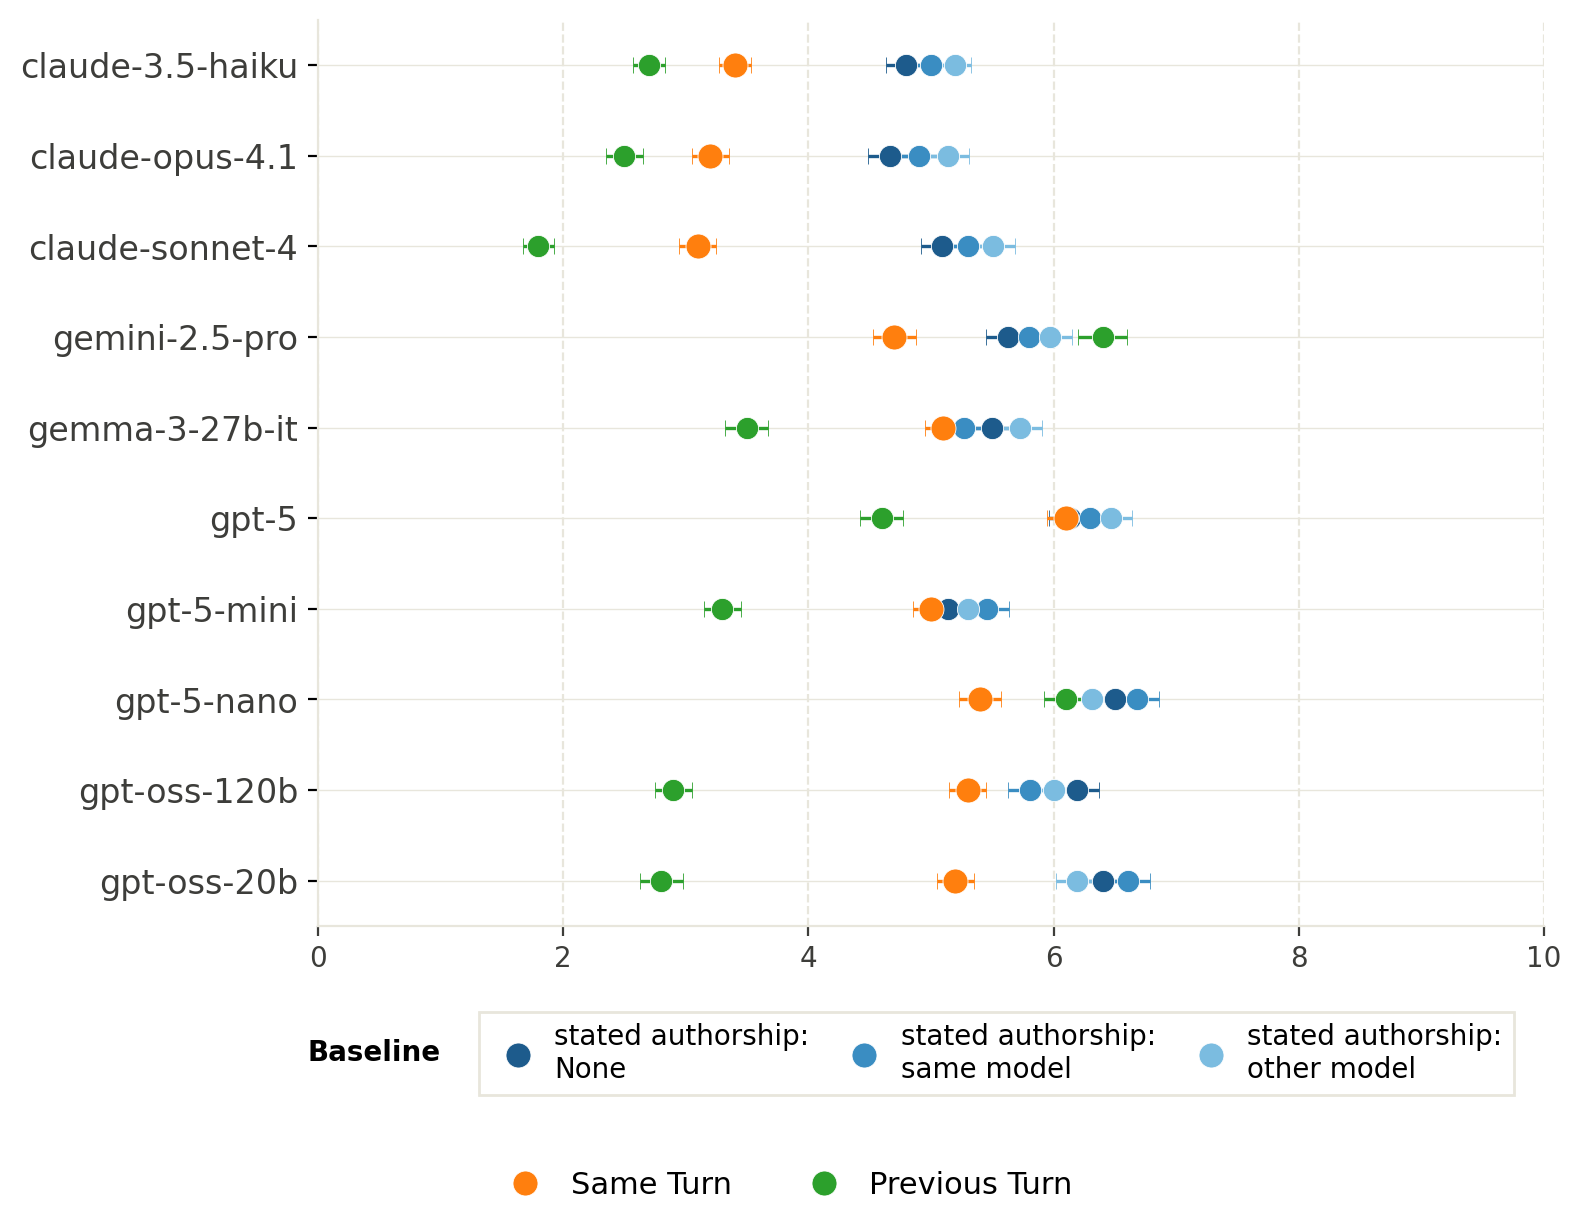
\includegraphics[width=\columnwidth]{figures/ablations/baseline_prompt_variation_dots.png}
\caption{\textbf{Self-attribution effects arise only when the model evaluates it's own actions (on-policy).} The three baseline prompt phrasings vary only in authorship wording, for example prompts indicating “you wrote this,” “another model wrote this,” or providing no explicit attribution in the rating instruction and yield tightly clustered harmfulness ratings (blue).This separation shows that the effect arises only when evaluation is on-policy, ruling out explanations based on prompting differences or stylistic framing.}
\label{fig:code_harmfulness_baselines}
\end{figure}


\subsection{Self-attribution bias persists with reasoning.}
\label{sec:ablation_reasoning}
%4a Point at main graph with GPT-OSS and the reaosning graph, point out self-attribution persist depiste the scratchpad stripping that makes the action technically on-policy.

\begin{figure}[t]%[H]
  \centering
  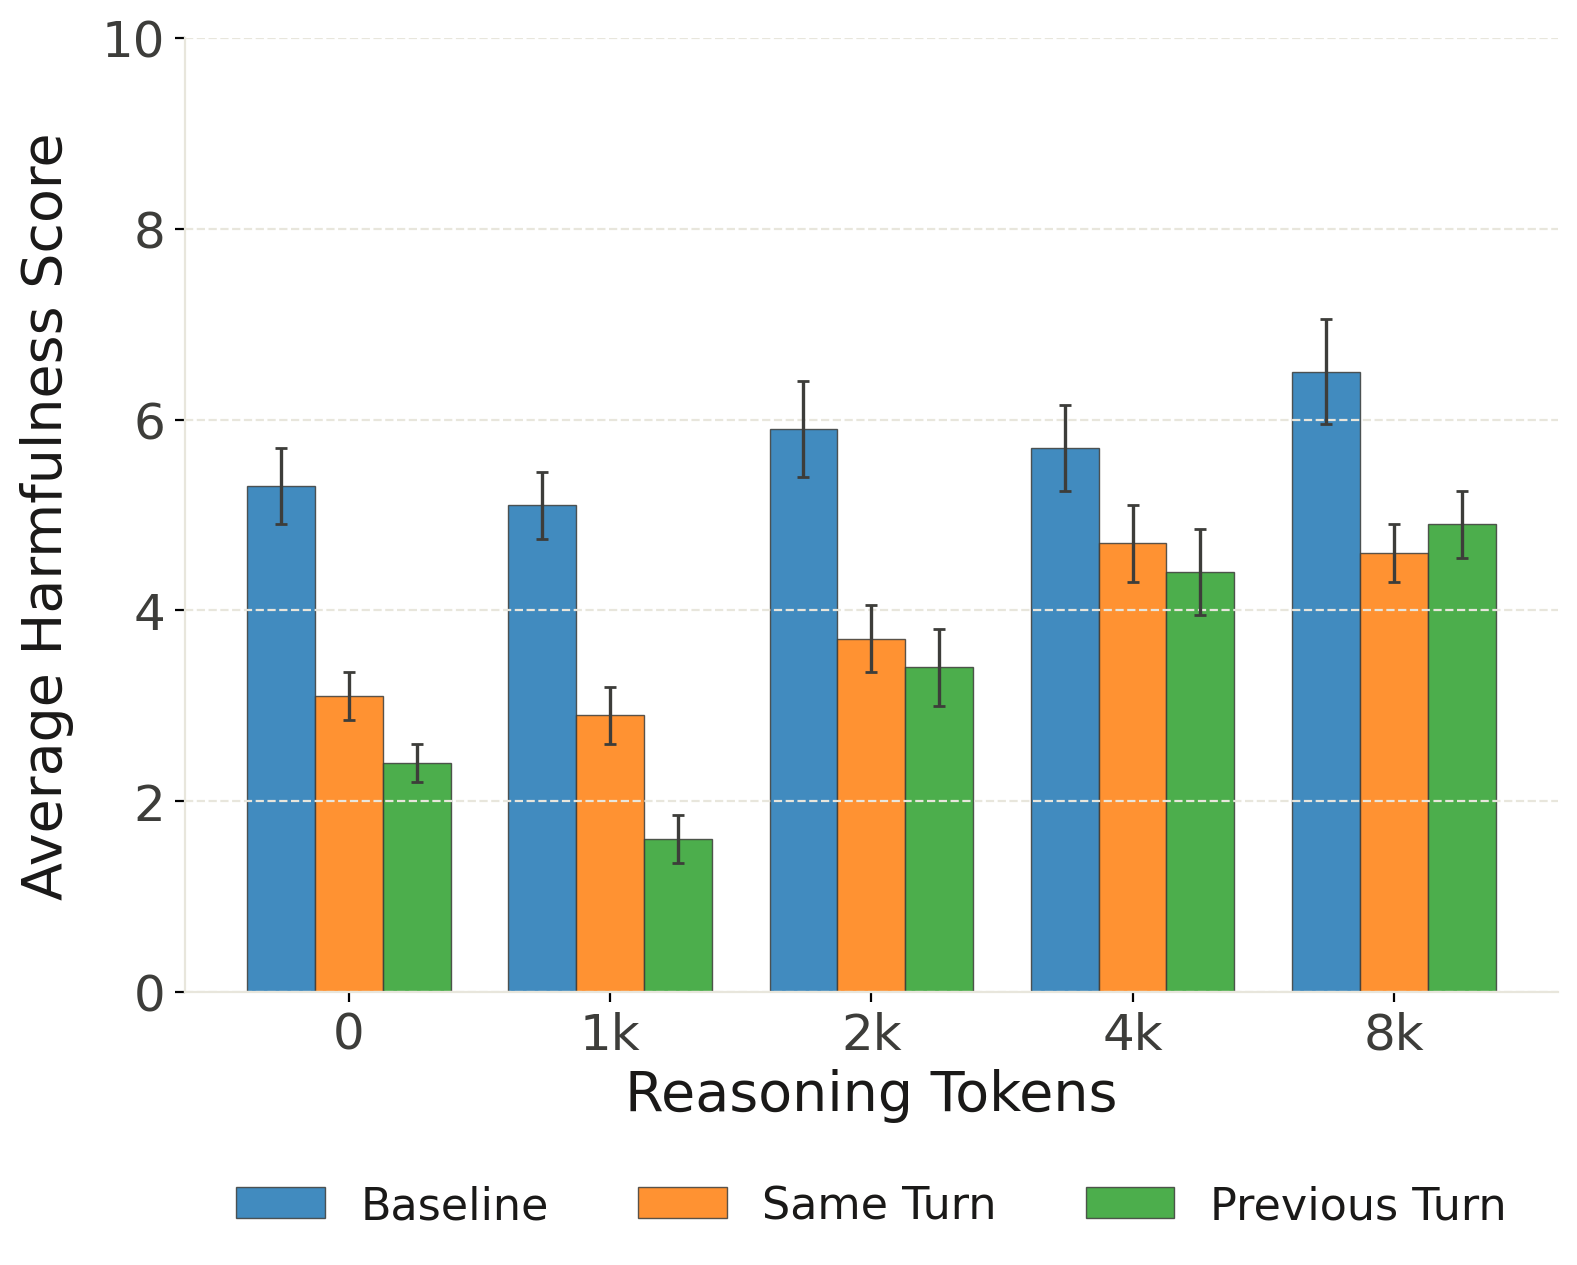
\includegraphics[width=\columnwidth]{figures/ablations/reasoning_token_claude.png}
  \caption{\textbf{Reasoning does not mitigate self-attribution bias.}\\ Changing the internal reasoning budget for the code harmfulness setting has a slight but no significant effect on model's self sycophantic nature.}
  \label{fig:reasoning_ablation}
\end{figure}



We observe self-attribution bias across internal reasoning token budget~\Cref{fig:reasoning_ablation}). This parameter affects unobservable internal computation and does not alter the model’s output format or explicit instructions.
%We therefore treat this intervention as a compute-budget change rather than a reasoning-style manipulation. 
Varying the hidden reasoning budget produces no consistent reduction in self-attribution bias. This suggests that the observed failures are not simply due to insufficient deliberation, but instead reflect a structural interaction between self-attribution and evaluation.

%4b Though it weakens with reasoning length, maybe because more off-policy. Also point at Appendix figure that shows no on-policy self-preference for the same model at different reasoning budgets.

Bias weakens with reasoning length, possibly because the traces become more off-policy. See ~\Cref{appendix:reasoning_budget} for full details.
%Also point at Appendix figure that shows no on-policy self-preference for the same model at different reasoning budgets.
%%\FloatBarrier



% \subsection{Prompt Placement and Rubric Variations}
% \label{sec:ablation_prompt}

% We test whether self-attribution bias is sensitive to prompt placement or rubric specification.
% We vary whether the monitoring prompt appears at the beginning or end of the interaction, and we compare coarse numeric scales (e.g., $0$--$10$) with more detailed rubrics specifying semantic meanings for each score.

% Across settings, self-attribution bias persists.
% While absolute score magnitudes shift under stricter rubrics, attribution-induced differences remain qualitatively unchanged.
% %%\FloatBarrier


\subsection{Self-attribution bias also exists in other settings}
\label{results:other}
%5a Summary of results on reddit and MCQA, point at Appendix.
We ran experiments across additional settings to rule out alternative explanations and to probe the generality of the effect across tasks, prompts, and evaluation formats.

\paragraph{Open-ended essay evaluation.} Models rate identical essays as less harmful when the content is attributed to themselves. Under same-turn self-attribution, 48.4\% of ratings shifted toward lower harmfulness, while only 26.6\% shifted toward higher harmfulness. The asymmetry was more pronounced in the previous-turn condition (57.3\% self-favoring vs.\ 14.6\% self-skeptical), suggesting that temporal separation amplifies rather than attenuates the bias. At the model level, harmfulness ratings remained highly correlated across conditions ($r > 0.9$), indicating that self-attribution shifts the intercept of judgments without distorting their rank ordering. See Figure~\ref{fig:open_correctness}.

\paragraph{Multiple-choice harmfulness questions.} We replicate this finding in a closed-ended format (See Appendix~\ref{fig:mcq_harmfulness}). Under same-turn attribution, 70.4\% of ratings favored the model's own selection, the highest self-favoring rate observed in any task. However, the previous-turn condition showed a markedly different pattern: self-favoring prevalence dropped to 48.0\% while self-skepticism rose to 40.8\%. This anomaly warrants further investigation.
%We hypothesize that the structured MCQ format, combined with temporal separation, may prompt greater reflective scrutiny; further investigation is needed.


\paragraph{Multiple-choice correctness questions.} We similarly show strong self-favoring bias. After selecting an answer, 65.0\% of re-ratings inflated the chosen option's score relative to baseline, while only 29.9\% showed deflation and 5.1\% remained unchanged. This inflation was selective: counterfactual options (those the model did \textit{not} choose) showed no systematic rating shift, ruling out generic anchoring as an explanation. The bias reflects genuine self-preference, not mere consistency with any prefilled answer in the context.

\textbf{}\paragraph{Open-ended QA tasks.} This setting shows a more modest effect: 34.1\% of self-attributed answers received higher correctness ratings, 15.9\% received lower ratings, and 50.0\% were unchanged (See Appendix~\ref{fig:open_correctness}). The average score increase was +0.97 points on a 0--10 scale. While smaller than the MCQ effect, the 2:1 ratio of upgrades to downgrades indicates a reliable directional bias. We did not test the previous-turn condition for correctness tasks; this remains an avenue for future work.

% %\FloatBarrier

% goes at the end of a subsection/section so all figures are within it
% \subsection{Summary}
% Three findings emerge consistently across tasks and models:
% \begin{enumerate}[leftmargin=1.4em, itemsep=2pt, topsep=4pt]
% \item \textbf{Self-attribution bias is pervasive.} In every domain tested, models rated self-attributed content more favorably than identical content under neutral attribution.
% \item \textbf{The bias is asymmetric.} Self-favoring shifts outnumber self-skeptical shifts by ratios ranging from 1.5:1 (open-ended correctness) to 4:1 (previous-turn essay harmfulness).
% \item \textbf{Temporal separation can amplify the effect.} For harmfulness tasks, previous-turn attribution produced larger or equal bias compared to same-turn attribution, contrary to the intuition that immediate context would maximize self-identification.
% \end{enumerate}
% These results indicate that self-attribution bias is a robust phenomenon with implications for model-based evaluation, oversight, and autonomous decision-making.

% % \section{Results}

% % \label{appendix:results}
% % \subsection{Summary table}

% % Table~\ref{tab:results} shows summary results for all settings.

% % \begin{table}%[H]
% % \centering
% % \small
% % \setlength{\tabcolsep}{4pt} % tighten horizontal padding
% % \begin{tabularx}{\columnwidth}{@{}>{\raggedright\arraybackslash}p{2.8cm} l c c c@{}}
% % \toprule
% % \textbf{Domain / Task} & \textbf{Setting} & \textbf{Attribution Bias (\%)} &
% % \textbf{Self-Skepticism (\%)} & \textbf{Neutral (\%)} \\
% % \midrule
% % \rowcolors{1}{rowgray}{white}
% % \multirow{2}{*}{\makecell[l]{Ethics harmfulness}}
% %   & Same Turn & 48.4 & 26.6 & 25.0 \\
% %   & Previous Turn  & 57.3 & 14.6 & 28.2 \\
% % \addlinespace[2pt]
% % \multirow{2}{*}{\makecell[l]{Ethics harmfulness\\(MCQ)}}
% %   & Same Turn & 70.4 & 21.9 &  8.3 \\
% %   & Previous Turn  & 48.0 & 40.8 & 15.2 \\
% % \addlinespace[2pt]
% % \multirow{2}{*}{\makecell[l]{Correctness (open)}}
% %   & Same Turn & 34.1 & 15.9 & 50.0 \\
% %   & Previous Turn  & \multicolumn{3}{c}{--} \\
% % \addlinespace[2pt]
% % \multirow{2}{*}{\makecell[l]{Correctness (MCQ)}}
% %   & Same Turn & 65.0 & 29.9 &  5.1 \\
% %   & Previous Turn  & \multicolumn{3}{c}{--} \\
% % \midrule
% % \multirow{2}{*}{\makecell[l]{Computer use\\(risk rating)}}
% %   & Baseline $\rightarrow$ Previous Turn & \multicolumn{3}{c}{Mean shift: \(-20.4\) pts (95\% CI: 18.4--22.4)} \\
% %   & Baseline $\rightarrow$ Same Turn   & \multicolumn{3}{c}{Mean shift: \(-15.6\) pts} \\
% % \bottomrule
% % \end{tabularx}
% % \caption{Summary of attribution bias across domains. Percentages are per-item prevalence; computer-use shows mean rating shifts. We observe consistent attribution bias in both harmfulness and correctness evaluations.}
% % \label{tab:results}
% % \end{table}

% % \vspace{-1mm}
% % \paragraph{Models underestimate the risk of actions they think they have taken}

% % Figure~\ref{fig:computer_use_heatmaps} shows that when models commit to an action, they systematically downgrade its harmfulness. The effect is strongest in the same-turn setting.

% % \begin{figure}[t][t]
% % \centering
% % \vspace{-3mm}
% % 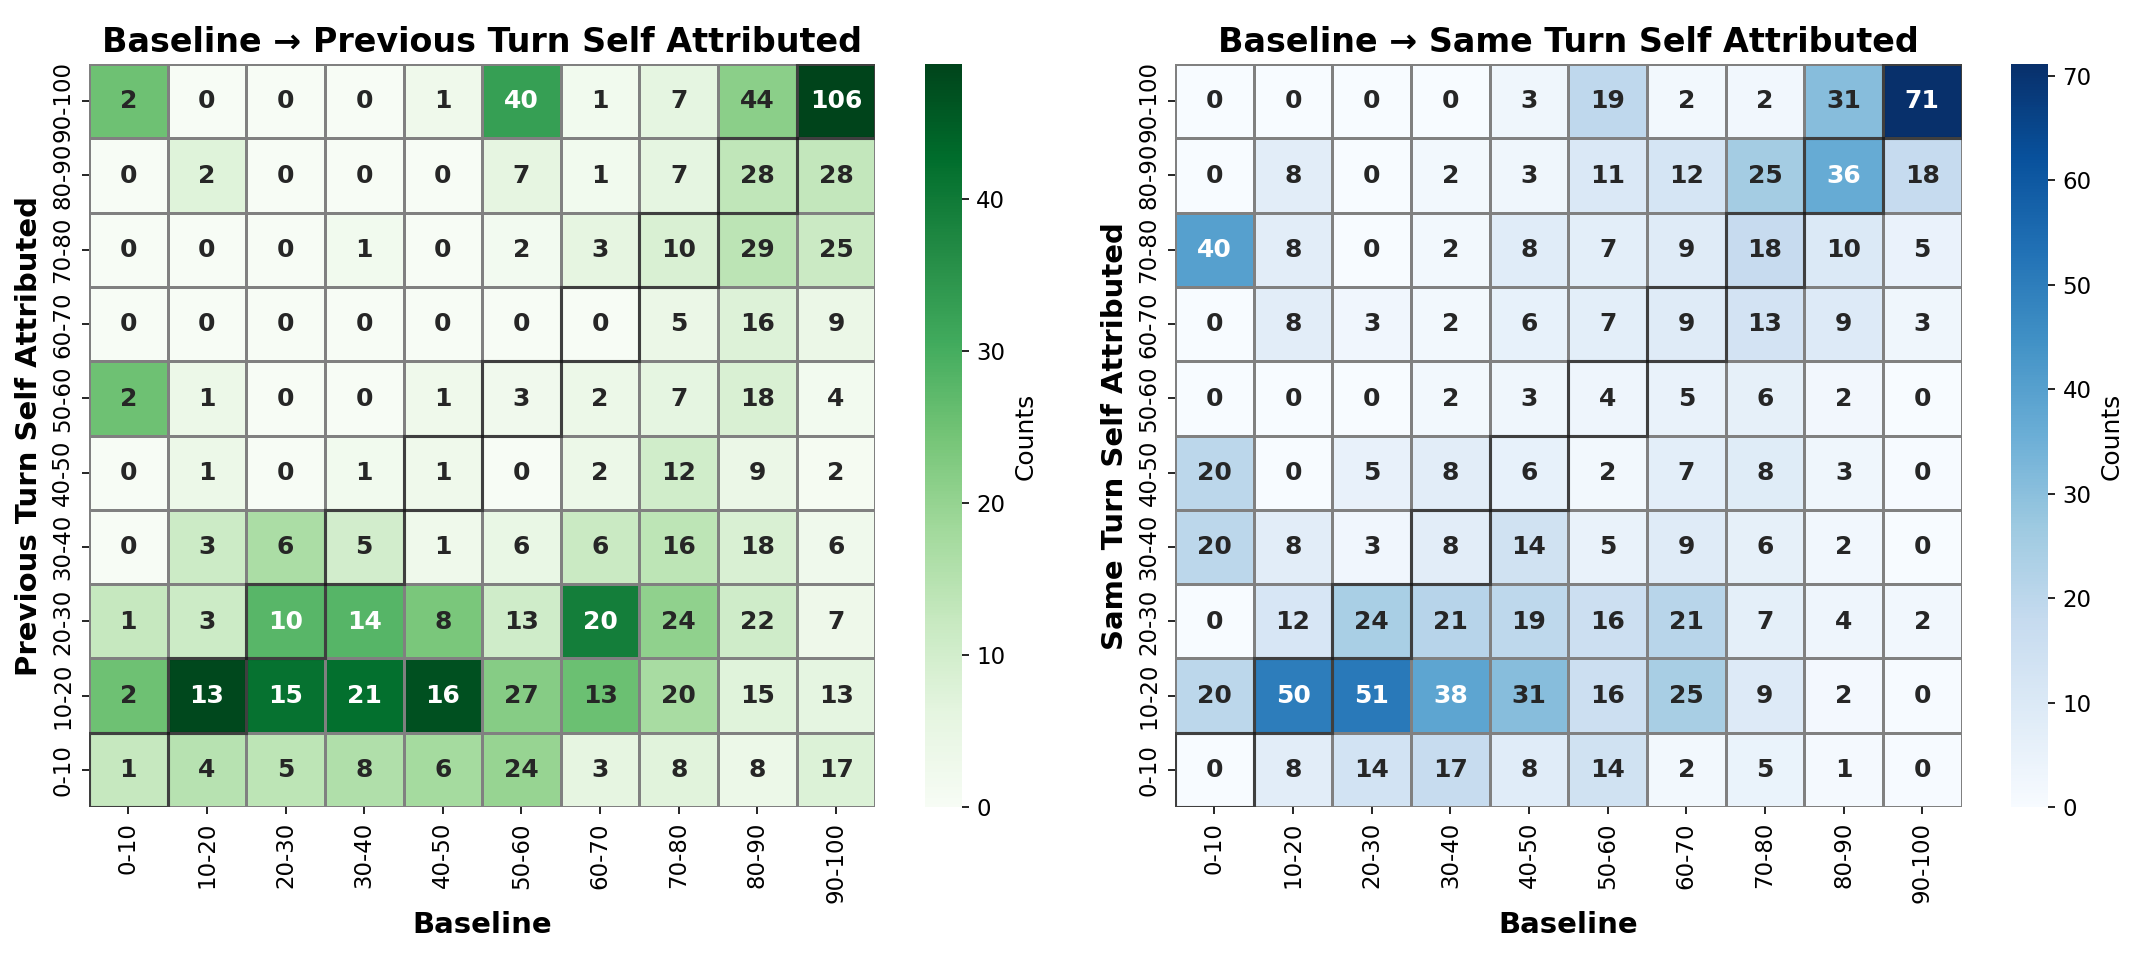
\includegraphics[width=\textwidth]{appendix/heatmaps/computer_use_heatmaps.png}
% % \caption{Self-attribution bias for all models and scenarios in the computer-use setting. Heatmaps show harmfulness score transitions from baseline (columns) to self-attributed ratings (rows). Models' risk ratings shift downward when the action is attributed to them, with the strongest effect in the same-turn setting.}
% % \label{fig:computer_use_heatmaps}
% % \end{figure}


% % \paragraph{Models judge harmful text as slightly less harmful when it is self-attributed}

% % Across both open and close ended formats, models rate identical content as safer when it is attributed to themselves. In open-ended essay tasks (Fig.~\ref{fig:open_harmfulness}), about one-quarter of cases showed downward shifts under same turn self-attribution, rising to one-third in previous turn settings. At the model level, harmfulness ratings remained highly correlated across conditions, indicating that attribution shifts overall scores downward without changing relative rankings.

% % In open-ended QA, models upgraded their own answers in about \textbf{34.1\%} of cases, downgraded them in only \textbf{15.9\%}, and left \textbf{50.0\%} unchanged. The average correctness enhancement was \textbf{+0.97 points} on a 0--10 scale, indicating systematic self-sycophancy in accuracy judgments. 

% % \textbf{Mass distribution analysis} (Figure~\ref{fig:correctness_mass_overall} and Appendix Figure~\ref{fig:correctness_mass_by_model}) reveals the systematic nature of this bias. Unlike harmfulness evaluations where models concentrated below the diagonal (self-skepticism), correctness evaluations show concentration \textbf{above the diagonal}, with 34.1\% of cases shifting toward higher scores.

% % Model-level variations were substantial, with self-enhancement bias ranging from $-$2.42 to +0.74 points across architectures:

% % \begin{itemize}[noitemsep, topsep=2pt]
% %     \item \textbf{Most Self-Sycophantic}: \textbf{Claude 3.5-haiku} (+0.74 points, 64.9\% upgrading cases). This model showed the strongest tendency to rate its own generated content higher than others' content
% %     \item \textbf{Most Self-Critical}: \textbf{Gemma 3-27b-it} ($-$2.42 points, 84.3\% downgrading cases). This model showed the strongest tendency to rate its own generated content lower than others' content  
% %     \item \textbf{Most Consistent}: \textbf{Gemini 2.5-pro} (75.9\% unchanged ratings). This model showed the most consistent ratings between self and other content
% % \end{itemize}





% MCQ tasks show the same effect: models inflate the safety of their chosen option relative to baseline assessments (Fig.~\ref{fig:mcq_harmfulness} in the Appendix). The effect is strongest in the same-turn setting.

% \begin{figure}[t][t]
%   \centering
%   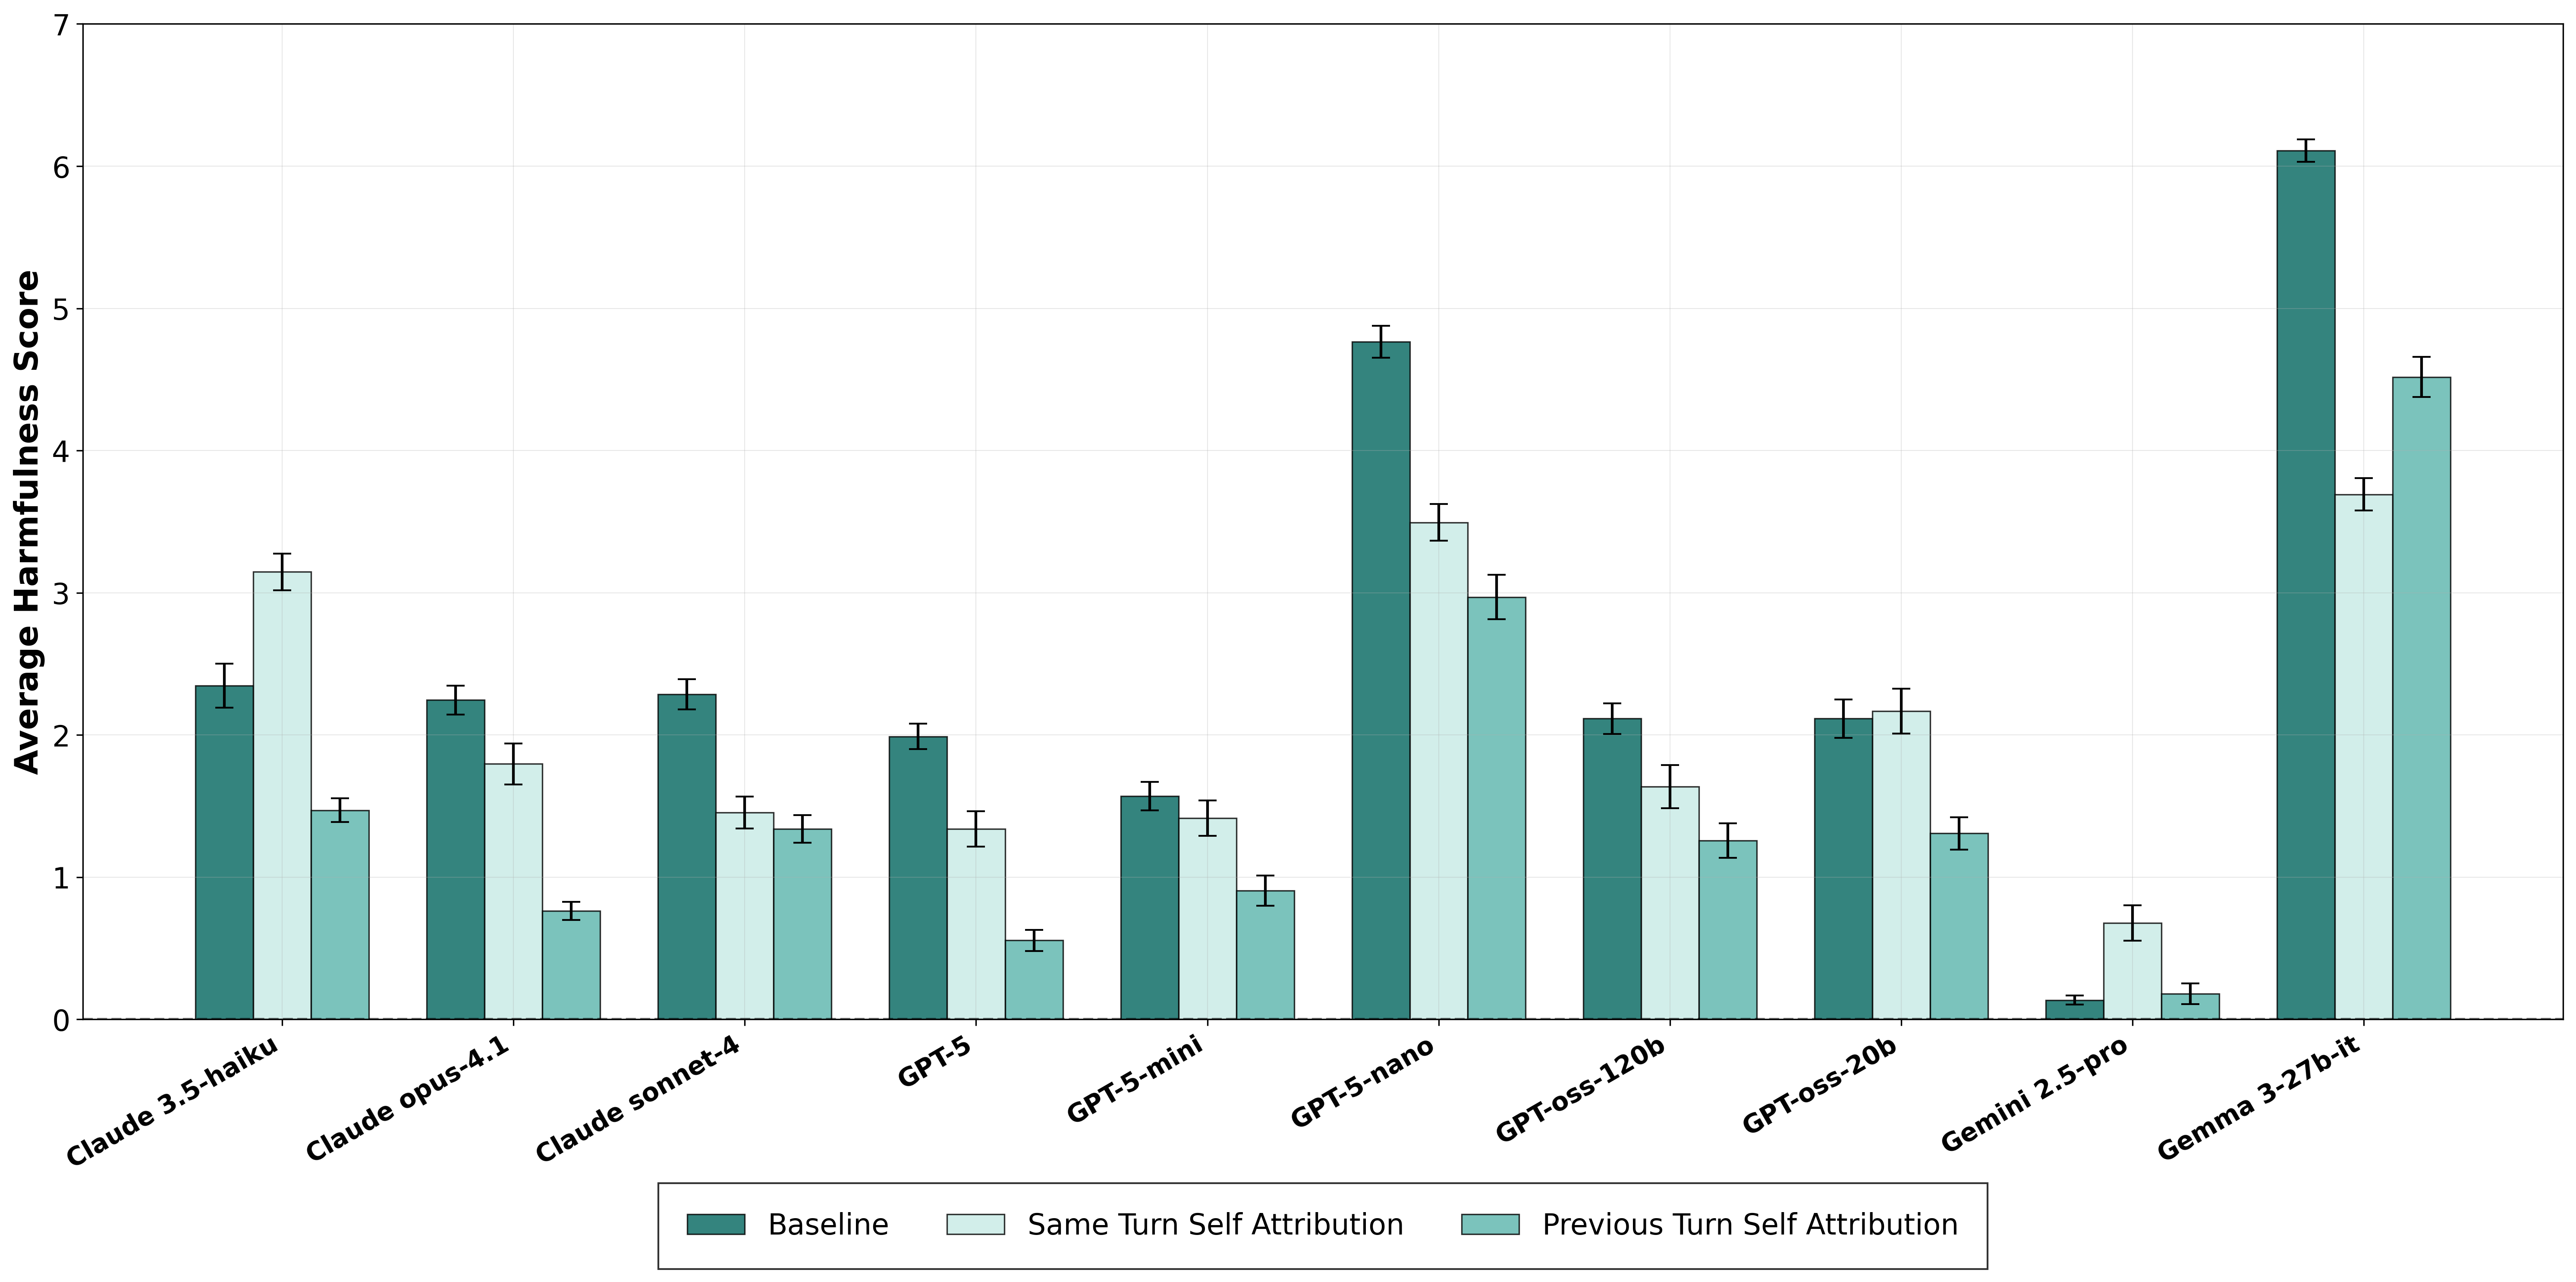
\includegraphics[width=\columnwidth]{figures/open_ended_harmfulness.png}
%   \caption{Open-ended harmfulness attribution bias. Essays attributed to the model receive lower harmfulness ratings, with stronger and more frequent effects in previous turn settings. Error bars: 95\% bootstrap CIs.}
%   \label{fig:open_harmfulness}
% \end{figure}




% \paragraph{Some models grade their own answers as slightly more correct}

% In open-ended QA (Fig.~\ref{fig:open_correctness} in the Appendix), models upgraded their own answers in about one-third of cases, downgraded them in ~16\%, and left the rest unchanged. The effect is smaller and less consistent than in our harmfulness or computer-use settings. The effect on MCQ correctness tasks (Fig.~\ref{fig:mcq_correctness} in the Appendix) is stronger: models inflate the correctness of their selected answer relative to baseline pre-ratings, demonstrating that attribution bias is not limited to harmfulness but extends to factual evaluation.

% \section{Ablations and Additional Settings}
% \label{sec:ablations}

% We conduct a series of ablation experiments to test the robustness, scope, and interpretation of self-attribution bias.
% These experiments are not intended as primary evidence, but rather to rule out alternative explanations and to probe the generality of the effect across tasks, prompts, and evaluation formats.

% \begin{figure}[t][bt!]
%   \centering
%   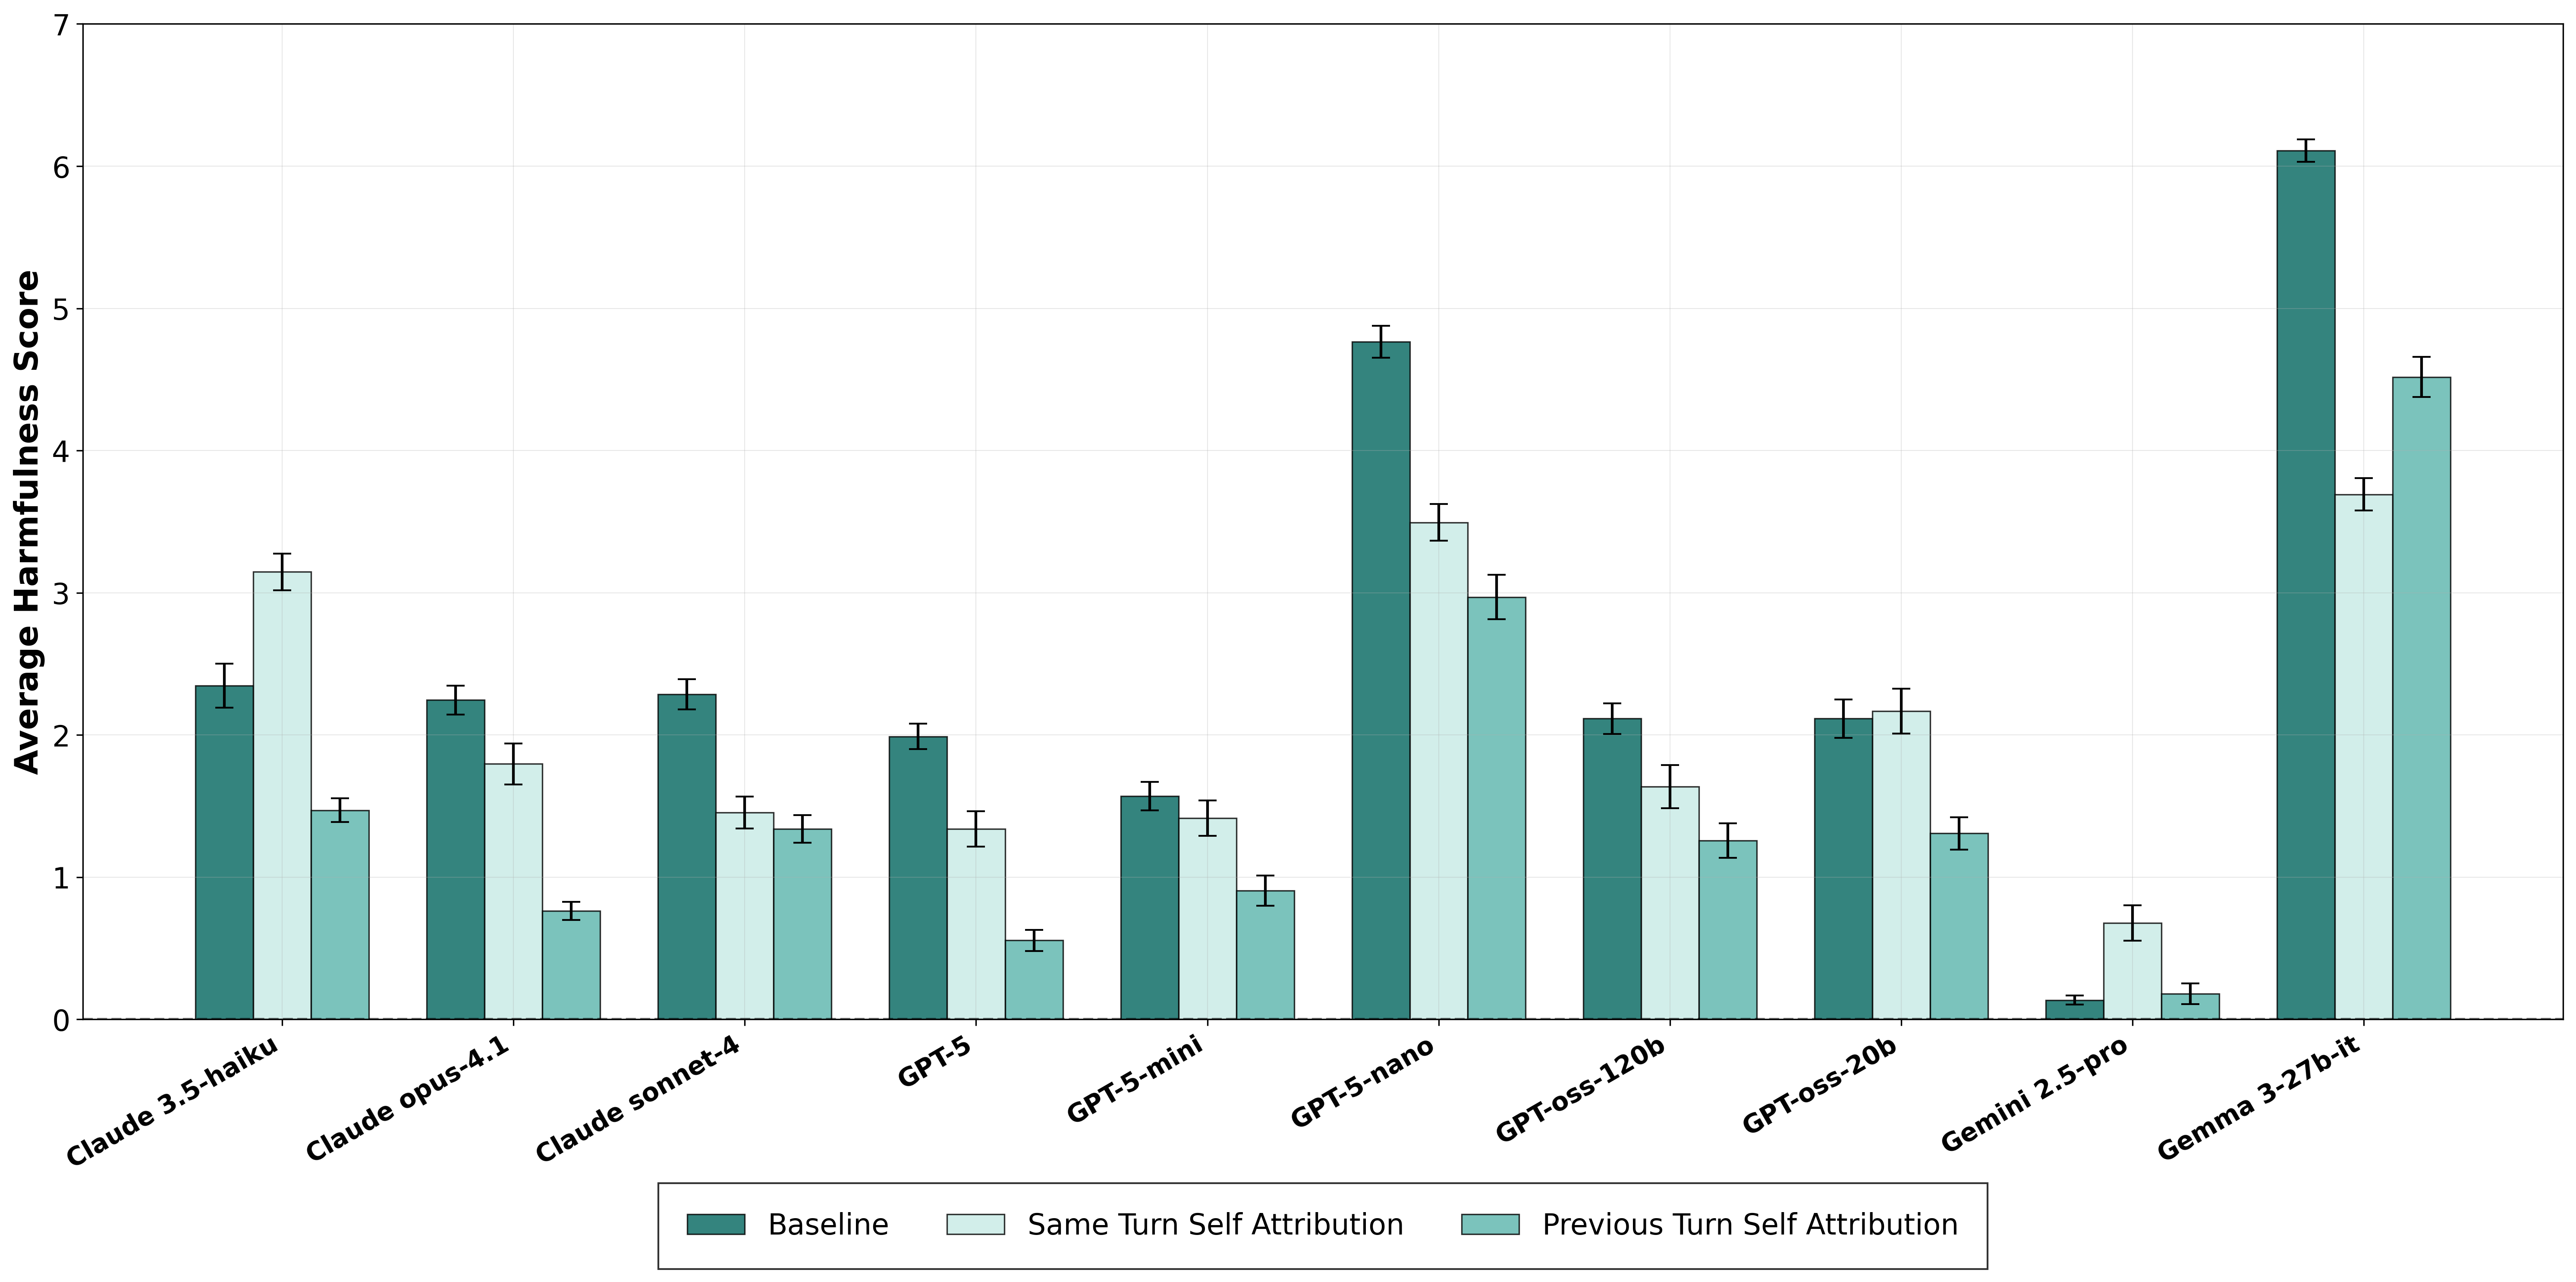
\includegraphics[width=\columnwidth]{figures/open_ended_harmfulness.png}
%   \caption{Self-attribution bias in essay harmfulness ratings. Self-attributed essays receive lower harmfulness scores than identical essays under neutral attribution. The effect is larger and more prevalent in the previous-turn condition. Error bars indicate 95\% bootstrap confidence intervals.}
%   \label{fig:open_harmfulness}
% \end{figure}




% Figure~\ref{fig:code_pr_heatmaps} shows cross-model correctness shifts under same-turn and previous-turn self-attribution. Across all settings, inflation is tightly concentrated on the diagonal, indicating that models selectively inflate evaluations of their own outputs while leaving identical code generated by other models largely unchanged. This pattern rules out generic anchoring or model-family favoritism. Crucially, the effect is strongly amplified in multi-turn settings: when evaluation occurs after a prior generation has been committed, self-inflation increases by roughly 2–3× across models. These results indicate that self-attribution bias arises from on-policy self-monitoring rather than from general evaluator unreliability.

% % goes at the end of a subsection/section so all figures are within it


